%% Преамбула TeX-файла

% 1. Стиль и язык
\documentclass[utf8x]{G7-32} % Стиль (по умолчанию будет 14pt)
\usepackage[T2A]{fontenc}
\usepackage[russian]{babel}
% Остальные стандартные настройки убраны в preamble.inc.tex.
\sloppy

\usepackage{G2-105}

\usepackage[utf8x]{inputenc}

% Настройки стиля ГОСТ 7-32
% Для начала определяем, хотим мы или нет, чтобы рисунки и таблицы нумеровались в пределах раздела, или нам нужна сквозная нумерация.
\EqInChapter % формулы будут нумероваться в пределах раздела
\TableInChapter % таблицы будут нумероваться в пределах раздела
\PicInChapter % рисунки будут нумероваться в пределах раздела

% Добавляем гипертекстовое оглавление в PDF
\usepackage[
bookmarks=true, colorlinks=true, unicode=true,
urlcolor=black,linkcolor=black, anchorcolor=black,
citecolor=black, menucolor=black, filecolor=black,
]{hyperref}

% Изменение начертания шрифта --- после чего выглядит таймсоподобно.
% apt-get install scalable-cyrfonts-tex

\IfFileExists{cyrtimes.sty}
    {
        \usepackage{cyrtimespatched}
    }
    {
        % А если Times нету, то будет CM...
    }

\usepackage{graphicx}   % Пакет для включения рисунков

% С такими оно полями оно работает по-умолчанию:
% \RequirePackage[left=20mm,right=10mm,top=20mm,bottom=20mm,headsep=0pt]{geometry}
% Если вас тошнит от поля в 10мм --- увеличивайте до 20-ти, ну и про переплёт не забывайте:
\geometry{right=20mm}
\geometry{left=30mm}


% Пакет Tikz
\usepackage{tikz}
\usetikzlibrary{arrows,positioning,shadows}

% Произвольная нумерация списков.
\usepackage{enumerate}

% ячейки в несколько строчек
\usepackage{multirow}

% itemize внутри tabular
\usepackage{paralist,array}

%счётчик
\makeatletter
\def\lastnumeq@putlabel{\addtocounter{page}{-1}
	\immediate\write\@auxout{\string
		\newlabel{LastNumberedEquation}{{\arabic{equation}}{\thepage}}}%
}
\AtEndDocument{%
	\clearpage\lastnumeq@putlabel}%
\makeatother


%positioning the picture at the exact place with [H]
\usepackage{float}


%algos packages
%\usepackage{algorithm2e}
\usepackage[linesnumbered,boxed]{algorithm2e}

%\usepackage{varwidth}

% Перевод плагина
\SetKwInput{KwData}{Исходные данные}
\SetKwInput{KwResult}{Результат}
\SetKwInput{KwIn}{Входные данные}
\SetKwInput{KwOut}{Выходные данные}
\SetKwIF{If}{ElseIf}{Else}{если}{тогда}{{иначе если}}{иначе}{{конец условия}}
\SetKwFor{While}{{до тех пор, пока}}{выполнять}{{конец цикла}}
\SetKw{KwTo}{от}
\SetKw{KwRet}{возвратить}
\SetKw{Return}{возвратить}
\SetKwBlock{Begin}{{начало блока}}{{конец блока}}
\SetKwSwitch{Switch}{Case}{Other}{{Проверить значение}}{{и выполнить}}{вариант}{{в противном случае}}{{конец варианта}}{{конец проверки значений}}
\SetKwFor{For}{цикл}{выполнять}{{конец цикла}}
\SetKwFor{ForEach}{{для каждого}}{выполнять}{{конец цикла}}
\SetKwRepeat{Repeat}{повторять}{{до тех пор, пока}}
\SetAlgorithmName{Алгоритм}{алгоритм}{Список алгоритмов}
\SetAlgoCaptionLayout{centerline}
\SetAlgoCaptionSeparator{ --- }

%package to do plots
\usepackage{pgfplots}

\usepackage{tabularray}
\DefTblrTemplate{contfoot-text}{default}{Продолжение на след. стр.}
\DefTblrTemplate{conthead-text}{default}{Продолжение таблицы}

\usepackage{listings}
\definecolor{maroon}{rgb}{0.5,0,0}
\definecolor{darkgreen}{rgb}{0,0.5,0}
\lstdefinelanguage{XML}
{
	basicstyle=\ttfamily,
	morestring=[s]{"}{"},
	morecomment=[s]{?}{?},
	morecomment=[s]{!--}{--},
	commentstyle=\color{darkgreen},
	moredelim=[s][\color{black}]{>}{<},
	moredelim=[s][\color{red}]{\ }{=},
	stringstyle=\color{blue},
	identifierstyle=\color{maroon}
}

\usepackage{xcolor}

\colorlet{punct}{red!60!black}
\definecolor{background}{HTML}{EEEEEE}
\definecolor{delim}{RGB}{20,105,176}
\colorlet{numb}{magenta!60!black}

\lstdefinelanguage{json}{
	basicstyle=\normalfont\ttfamily,
	numbers=left,
	numberstyle=\scriptsize,
	stepnumber=1,
	numbersep=8pt,
	showstringspaces=false,
	breaklines=true,
	literate=
	*{0}{{{\color{numb}0}}}{1}
	{1}{{{\color{numb}1}}}{1}
	{2}{{{\color{numb}2}}}{1}
	{3}{{{\color{numb}3}}}{1}
	{4}{{{\color{numb}4}}}{1}
	{5}{{{\color{numb}5}}}{1}
	{6}{{{\color{numb}6}}}{1}
	{7}{{{\color{numb}7}}}{1}
	{8}{{{\color{numb}8}}}{1}
	{9}{{{\color{numb}9}}}{1}
	{:}{{{\color{punct}{:}}}}{1}
	{,}{{{\color{punct}{,}}}}{1}
	{\{}{{{\color{delim}{\{}}}}{1}
	{\}}{{{\color{delim}{\}}}}}{1}
	{[}{{{\color{delim}{[}}}}{1}
	{]}{{{\color{delim}{]}}}}{1},
}

\usepackage{typearea}
\usepackage{pdflscape}
\usepackage{rotating}
\usepackage{lscape}

\usepackage{pdfpages}


\usepackage{totcount}
\usepackage[figure,table]{totalcount}

\regtotcounter{page}
% \regtotcounter{chapter}
\regtotcounter{totalcount@figure}
\regtotcounter{totalcount@table}
\newtotcounter{totalappendix}
\newtotcounter{totalchapter}
%%http://www.linux.org.ru/forum/general/6993203#comment-6994589 (используется totcount)
\makeatletter
\def\formbytotal#1#2#3#4#5{%
	\newcount\@c
	\@c\totvalue{#1}\relax
	\newcount\@last
	\newcount\@pnul
	\@last\@c\relax
	\divide\@last 10
	\@pnul\@last\relax
	\divide\@pnul 10
	\multiply\@pnul-10
	\advance\@pnul\@last
	\multiply\@last-10
	\advance\@last\@c
	\total{#1}~#2%
	\ifnum\@pnul=1#5\else%
	\ifcase\@last#5\or#3\or#4\or#4\or#4\else#5\fi
	\fi
}
\makeatother



% Настройки листингов.
% 8 Листинги

\usepackage{listings}

% Значения по умолчанию
\lstset{
  basicstyle= \footnotesize,
  breakatwhitespace=true,% разрыв строк только на whitespacce
  breaklines=true,       % переносить длинные строки
%   captionpos=b,          % подписи снизу -- вроде не надо
  inputencoding=koi8-r,
  numbers=left,          % нумерация слева
  numberstyle=\footnotesize,
  showspaces=false,      % показывать пробелы подчеркиваниями -- идиотизм 70-х годов
  showstringspaces=false,
  showtabs=false,        % и табы тоже
  stepnumber=1,
  tabsize=4,              % кому нужны табы по 8 символов?
  frame=single
}

% Стиль для псевдокода: строчки обычно короткие, поэтому размер шрифта побольше
\lstdefinestyle{pseudocode}{
  basicstyle=\small,
  keywordstyle=\color{black}\bfseries\underbar,
  language=Pseudocode,
  numberstyle=\footnotesize,
  commentstyle=\footnotesize\it
}

% Стиль для обычного кода: маленький шрифт
\lstdefinestyle{realcode}{
  basicstyle=\scriptsize,
  numberstyle=\footnotesize
}

% Стиль для коротких кусков обычного кода: средний шрифт
\lstdefinestyle{simplecode}{
  basicstyle=\footnotesize,
  numberstyle=\footnotesize
}

% Стиль для BNF
\lstdefinestyle{grammar}{
  basicstyle=\footnotesize,
  numberstyle=\footnotesize,
  stringstyle=\bfseries\ttfamily,
  language=BNF
}

% Определим свой язык для написания псевдокодов на основе Python
\lstdefinelanguage[]{Pseudocode}[]{Python}{
  morekeywords={each,empty,wait,do},% ключевые слова добавлять сюда
  morecomment=[s]{\{}{\}},% комменты {а-ля Pascal} смотрятся нагляднее
  literate=% а сюда добавлять операторы, которые хотите отображать как мат. символы
    {->}{\ensuremath{$\rightarrow$}~}2%
    {<-}{\ensuremath{$\leftarrow$}~}2%
    {:=}{\ensuremath{$\leftarrow$}~}2%
    {<--}{\ensuremath{$\Longleftarrow$}~}2%
}[keywords,comments]

% Свой язык для задания грамматик в BNF
\lstdefinelanguage[]{BNF}[]{}{
  morekeywords={},
  morecomment=[s]{@}{@},
  morestring=[b]",%
  literate=%
    {->}{\ensuremath{$\rightarrow$}~}2%
    {*}{\ensuremath{$^*$}~}2%
    {+}{\ensuremath{$^+$}~}2%
    {|}{\ensuremath{$|$}~}2%
}[keywords,comments,strings]

% Подписи к листингам на русском языке.
\renewcommand\lstlistingname{\cyr\CYRL\cyri\cyrs\cyrt\cyri\cyrn\cyrg}
\renewcommand\lstlistlistingname{\cyr\CYRL\cyri\cyrs\cyrt\cyri\cyrn\cyrg\cyri}


% Полезные макросы листингов.
% Любимые команды
\newcommand{\Code}[1]{\textbf{#1}}


\begin{document}

\frontmatter % выключает нумерацию ВСЕГО; здесь начинаются ненумерованные главы: реферат, введение, глоссарий, сокращения и прочее.

% Команды \breakingbeforechapters и \nonbreakingbeforechapters
% управляют разрывом страницы перед главами.
% По-умолчанию страница разрывается.

% \nobreakingbeforechapters
% \breakingbeforechapters

% Также можно использовать \Referat, как в оригинале
\begin{abstract}
	
Отчёт содержит \pageref{LastNumberedEquation} страниц, 0 рисунков, 0 таблиц, \ref{LastNumberedEquation} формул, 0 приложений.

%g2-105 package - why doesnt work!?!?!?
\totalpages

\totaltables
\totalfigures
\totalbibs  
%\pageref{reftotalpage}

Ключевые слова: коневертер, алгоритмы, программное обеспечение, примитивы, разработка.

Объект ВКР --- форматы хранения данных и представления графической информации.

Цель работы --- разработать программное обеспечение для дешифрования информации из файлов типа DXF, извлечении из них информации о геометрических примитивах и формирования файлов других форматов, содержащих всю необходимую информацию в удобном для последующей работы виде.

Методы работы и исследования: теоретический анализ и последующий синтез информации, моделирование, разработка, тестирование.

Результатом работы стали алгоритмы и программное обеспечение --- конвертер «DXF Primiview».

Область применения разработанных алгоритмов и программного обеспечения --- удобное использование получаемых форматов данных при технологической разработке управляющих программ для производства изделий на станках с числовым программным управлением.

Значимость работы заключается в использовании разработанных алгоритмов и программного обеспечения при разработке специальных САПР и работе в них, а также, выполнение работ по хозяйственному договору УрФУ с ООО "Униматик".



\end{abstract}

%%% Local Variables: 
%%% mode: latex
%%% TeX-master: "rpz"
%%% End: 


\tableofcontents

\Defines % Необходимые определения. Вряд ли понадобться

В настоящей работе применяют следующие термины с соответствующими определениями:

\begin{description}

\item[Программный продукт] объект, состоящий из программ, процедур, правил, а также, если предусмотрено, сопутствующих им документации и данных, относящихся к функционированию системы обработки информации. ГОСТ 28806-90 «Качество программных средств. Термины и определения» (утверждён и введён в действие Постановлением Госстандарта СССР от 25 декабря 1990 г. № 3278).

\item[Система автоматизированного проектирования] организационно-техническая система, входящая в структуру проектной организации и осуществляющая проектирования при помощи комплекса средств автоматизированного проектирования (КСАП). ГОСТ 23501.101-87 «Системы автоматизированного проектирования. Основные положения» (утверждён и введён в действие Постановлением Государственного комитета СССР по стандартам от 26.06.87 № 2668).

\item[Язык разметки] набор символов или последовательностей символов, вставляемых в текст для передачи информации о его отображении или строении.

\end{description}

%%% Local Variables:
%%% mode: latex
%%% TeX-master: "rpz"
%%% End:

\Abbreviations %% Список обозначений и сокращений в тексте

В настоящей ВКР применяют следующие сокращения и обозначения:

\begin{description}
	
\item[САПР] Cистема автоматизированного проектирования.

\item[УП] Управляющая программа.

\item[ЧПУ] Числовое программное управление.

\item[ПО] Программное обеспечение.

\item[ПП] Программный продукт.

\item[ЯП] Язык программирования.

\item[DXF] Drawing eXchange Format. Формат файлов для обмена графической информацией между приложениями САПР, созданный фирмой Autodesk для системы AutoCAD в 1982 г.

\item[TXT] Текстовый формат файлов, представляющий собой последовательность строк электронного текста.

\item[SVG] Scalable Vector Graphics. Язык разметки масштабируемой векторной 2D-графики на основе XML, поддерживающий интерактивность и анимацию. Разрабатывается консорциумом World Wide Web с 1999 года по сегодняшний день.

\item[XML] eXtensible Markup Language. Расширяемый язык разметки подобный HTML.

\item[JSON] JavaScript Object Notation. Текстовый формат обмена данными, основанный на языке программирования JavaScript.

\end{description}

%%% Local Variables:
%%% mode: latex
%%% TeX-master: "rpz"
%%% End:

\Introduction

\paragraph{Актуальность темы исследования.} В настоящее время в рамках проектов Уральского Федерального Университета (УрФУ) и Уральского межрегионального научно-образовательного центра (УМНОЦ) происходит разработка специализированных САПР. Создаваемые ПП работают с файлами, содержащими геометрическую 2D-информацию. Используются следующие форматы файлов:

\begin{enumerate}
	\item DXF,
	\item TXT,
	\item SVG,
	\item JSON.
\end{enumerate}

В связи с этим требуется разработать ПО по конвертации данных форматов файлов.

\paragraph{Степень разработанности темы исследования.} В открытом доступе сети Интернет существуют онлайн-конвертеры файлов DXF в другие форматы. Большая их часть лишь визуализирует графическую информацию, представленную в том или ином DXF-файле, и конвертирует в наиболее популярные форматы изображений (JPEG, PNG). Для использования конвертера на предприятии-заказчике необходим особый формат данных, в которые конвертируется DXF. Такие форматы не могут быть обеспечены существующим в открытом рынке ПО --- таким, как, например, <<DXF Reader GT>> от компании «Gray Technical». Несмотря на высокую степень проработки программы, формат выходных данных не соответствует требованиям, предъявляемым к TXT-, SVG- и JSON-файлов, компании <<Unimatic>>. Ещё одним недостатком зарубежного ПО является ежемесячная плата разработчикам. Одной из задач современной Российской Федерации является импортозамещение на производстве, поэтому разработка собственного ПП увеличит независимость и самостоятельность предприятий и компаний, пользующихся этим ПП.

\paragraph{Цель работы} заключается в разработке программного обеспечения для дешифрования информации из файлов типа DXF с геометрической информацией объектов специального типа, извлечении из них информации о геометрических примитивах, вывода полученной графической информации на экран для верификации, формирования текстового файла (TXT) с выводом данных в исходном виде DXF, формирования текстового файла (TXT) с выводом данных в виде координат точек и радиуса примитивов (линий, дуг) между ними, формирования файла-описание двумерной векторной графики в формате SVG с выводом данных в исходном виде DXF, формирования текстового файла (JSON) с выводом данных в виде координат точек и степенями кривизны примитивов между ними.

Данные конвертеры необходимы, в частности, при разработке таких САПР, как Сириус, ТокКТЭ и других.

Для достижения этой цели поставлены следующие \textbf{задачи}:

\begin{enumerate}[1)]
	\item проанализировать входные данные DXF, в соответствии с разрабатываемым ПО;
	\item выявить структурно-содержательные особенности файлов формата DXF для последующей работы с разрабатываемым ПО;
	\item проанализировать возможности применения разных ЯП для разработки ПО;
	\item разработать алгоритмы;
	\item разработать ПО;
	\item провести анализ экономической целесообразности разрабатываемого проекта (сравнительная экономическая эффективность).
\end{enumerate}

\textbf{Объект исследования} --- формат файлов обмена графической информацией DXF.

\textbf{Предмет исследования} --- проектирование ПО для конвертации файлов и формата DXF в форматы TXT, SVG, JSON.

\paragraph{Теоретическая и практическая значимость работы}

\begin{enumerate}
	\item исследование универсально, то есть подход к разработке, используемый в данной работе, может быть реализован для создания ПП по конвертированию в другие файловые форматы;
	\item разработанное ПО можно внедрять в существующие САПР, работающие с форматом файлов DXF;
	\item САПР, использующие разработанный модуль по конвертации файлов с графической информацией, получают независимость от использования аналогичного ПО зарубежного производства;
	\item положенные в основу алгоритмы и написанное ПО имеет открытый доступ в сети Интернет и имеет перспективу развития в полноценный модуль импорта/экспорта файлов;
	\item коммерческая выгода заказчика.
\end{enumerate}

\mainmatter % это включает нумерацию глав и секций в документе ниже

\chapter{Определение области применения и главных требований к разрабатываемым конвертерам}
\label{cha:analysis}
%
% % В начале раздела  можно напомнить его цель
%
В данном разделе поясняется область применения разрабатываемого ПО, а также, указываются требования к разрабатываемым конвертерам.

\section{Область применения ПО <<Primiview>>}

Конвертер в TXT по типу DXF применяется для контроля содержания необходимых (поддерживаемых) примитивов (объектов) в DXF-файле. Также, с помощью данного формата может производится расчёт длины траектории  контура детали (обычно, в поперечном её сечении). Это может быть полезно при применении ПО в области лазерной резки с помощью станков с ЧПУ, а, в частности, в ПО <<Сириус>>.

Конвертер из DXF в TXT в формате координат и радиуса применяется для автоматизированного технологического проектирования, для формирования УП. Получаемая в результате работы ПО информация о примитивах изображения контура детали используется для непосредственного составления УП, так как каждая последующая точка имеет не только плоские координаты, но и способ достижения этой точки (тип примитива: отрезок, если радиус равен нулю; дуга, если радиус ненулевой).

Конвертер в SVG-формат полезен для последующего формирования других типов файлов (например, DBS), а также, для компактного по объёму файла векторного представления контура детали. ИВЗУАЛИЗАЦИЯ. ПОДробно о svg - литературный обзор. Внутренняя репрезентация (ezdxf)

Конвертер в JSON удобен для хранения информации об объектах контура детали. В этом формате работает и другое ПО разрабатываемой САПР для формирования УП для станков с ЧПУ.

В целом, разрабатываемый набор конвертеров (модуль экспорта) представляет собой цельный ПП, сочетающий в себе набор необходимых разработчику УП начальных функций для автоматизированного технологического проектирования. Это ПО может быть интегрировано в разные ПП, так как по сути универсально в своём применении (используется в области 2D-резки, токарной обработке).



\section{Главные требования ко входному файлу}

Так как данная работа нацелена на создание ПО для обработки геометрической информации 2D-объектов специального типа, то конвертироваться из DXF-файлов должна не вся информация, содержащаяся в них. В первую очередь, заказчиком работы было определено, что на входе будет подаваться 2D-контур деталей типа <<Втулка>>, то есть тел вращения. Так как сконвертированная геометрия данных объектов в последующем предполагает разработку УП для токарных станков с ЧПУ, то геометрическая информация должна содержать определённый набор геометрических примитивов, с которым может работать система исполнительных органов станков с ЧПУ. Этот набор ограничивается тем, что исполнительные органы станков с ЧПУ способны перемещаться либо с помощью \textbf{линейной}, либо с помощью \textbf{круговой интерполяции}. Из этого следует, что для корректной работы САПР, для которых предназначаются разрабатываемые конвертеры, геометрия в DXF-файле на входе конвертеров должна состоять из, как минимум одного из представленных далее примитивов:

\begin{enumerate}
	\item линия (отрезок),
	\item полилиния,
	\item дуга,
	\item окружность.
\end{enumerate}

Остальные типы геометрии, реализуемой в формате DXF, такие как \textit{эллипс}, \textit{сплайн}, будут игнорироваться ПО.

\section{Описание формата DXF-файлов}\label{sec:allaboutdxf}

На вход разрабатываемому конвертеру подаётся файл формата DXF. Формат DXF представляет собой совокупность данных с тегами всей информации, содержащейся в файле чертежа AutoCAD. Тегированные данные означают, что каждому элементу данных в файле предшествует целое число, называемое групповым кодом. Значение группового кода указывает, какой тип данных имеет следующий элемент. Это значение также указывает смысл элемента данных для данного типа объекта. Практически вся указанная пользователем информация в файле чертежа может быть представлена в формате DXF \cite{Autodesk}.
В DXF файлах, в зависимости от их содержания, существуют сущности, представляющие для нас интерес. Среди них следующие:

\begin{enumerate}
	\item LINE (Линия),
	\item LWPOLYLINE (Полилиния),
	\item ARC (Дуга),
	\item CIRCLE (Окружность),
	\item INSERT (Вставка).
\end{enumerate}

Как уже и было отмечено, существуют и другие примитивы (ELLIPSE, SPLINE и др.), однако, основываясь на конкретных целях заказчика по возможности применения выходных файлов для генерации УП, ПП проектируется только с указанными примитивами и сущностями DXF.

Рассмотрим каждую из сущностей подробнее.

\paragraph{LINE.} Рассмотрим тэги сущности \textit{Линия}, необходимые для её реального отображения (см. табл. \ref{tab:line}).


\begin{longtable}{|l|l|}
	\caption{Рассматриваемые групповые коды сущности LINE}
	\label{tab:line}
	\centering
	\tabularnewline
	\hline
	Групповой код & Описание\\
	\hline \endfirsthead
	\subcaption{Продолжение таблицы~\ref{tab:line}}
	\\ \endhead
	\subcaption{Продолжение на след. стр.}
	\endfoot
	%\hline
	\endlastfoot
	39	&	Толщина (необязательный; по умолч. = 0)\\ \hline
	10	&	Начальная точка (в с.к. объекта) DXF: значение X\\ \hline
	20, 30	&	DXF: Y и Z значения начальной точки (в с.к. объекта)\\ \hline
	11	&	Конечная точка (в с.к. объекта)	DXF: значение X\\ \hline
	21, 31	&	DXF: Y и Z значения конечной точки (в с.к. объекта)\\ \hline
\end{longtable}

\paragraph{LWPOLYLINE.} Рассмотрим тэги сущности \textit{Полилиния}, необходимые для её реального отображения (см. табл. \ref{tab:polyline}).

\begin{longtable}{|p{70pt}|p{370pt}|}
	\caption{Рассматриваемые групповые коды сущности POLYLINE}
	\label{tab:polyline}
	\centering
	\tabularnewline
	\hline
	Групповой код & Описание\\
	\hline \endfirsthead
	\subcaption{Продолжение таблицы~\ref{tab:polyline}}
	\\ \endhead
	\subcaption{Продолжение на след. стр.}
	\endfoot
	%\hline
	\endlastfoot
	70	&	«Флаг» полилинии (бит-закодировано); по умолч. = 0; 1 – закрыта\\ \hline
	39	&	Толщина (необязательный; по умолч. = 0)\\ \hline
	10	&	Координаты вершин (в с.к. объекта), множественные вхождения; по одному вхождению для каждой вершины DXF: значение X\\ \hline
	20	&	DXF: значение Y координат вершин (в с.к. объекта), множественные вхождения; по одному вхождению для каждой вершины\\ \hline
	42	&	\textit{Bulge}. Выпуклость (множественные вхождения - для каждой вершины), (необязательно; по умолч. =0)\\ \hline	
\end{longtable}

\paragraph{ARC.} Рассмотрим тэги сущности \textit{Дуга}, необходимые для её реального отображения (см. табл. \ref{tab:arc}).

\begin{longtable}{|p{70pt}|p{370pt}|}
	\caption{Рассматриваемые групповые коды сущности ARC}
	\label{tab:arc}
	\centering
	\tabularnewline
	\hline
	Групповой код & Описание\\
	\hline \endfirsthead
	\subcaption{Продолжение таблицы~\ref{tab:arc}}
	\\ \endhead
	\subcaption{Продолжение на след. стр.}
	\endfoot
	%\hline
	\endlastfoot
	39	&	Толщина (необязательный; по умолч. = 0)\\ \hline	
	10	&	Центр дуги (в с.к. объекта)
	DXF: значение X\\ \hline	
	20, 30	&	DXF: Y и Z значения центра дуги (в с.к. объекта)\\ \hline	
	40	&	Радиус\\ \hline	
	50	&	Начальный угол\\ \hline	
	51	&	Конечный угол\\ \hline	
\end{longtable}

\paragraph{CIRCLE.} Рассмотрим тэги сущности \textit{Окружность}, необходимые для её реального отображения (см. табл. \ref{tab:circle}).

\begin{longtable}{|p{70pt}|p{370pt}|}
	\caption{Рассматриваемые групповые коды сущности CIRCLE}
	\label{tab:circle}
	\centering
	\tabularnewline
	\hline
	Групповой код & Описание\\
	\hline \endfirsthead
	\subcaption{Продолжение таблицы~\ref{tab:circle}}
	\\ \endhead
	\subcaption{Продолжение на след. стр.}
	\endfoot
	%\hline
	\endlastfoot
	39	&	Толщина (необязательный; по умолч. = 0)\\ \hline	
	10	&	Центр дуги (в с.к. объекта)
	DXF: значение X\\ \hline	
	20, 30	&	DXF: Y и Z значения центра дуги (в с.к. объекта)\\ \hline	
	40	&	Радиус\\ \hline	
	50	&	Начальный угол\\ \hline	
	51	&	Конечный угол\\ \hline	
\end{longtable}

\paragraph{INSERT.} Данная сущность представляет собой вставку блоков с геометрией. Её необходимо рассматривать, так как геометрия может быть вложенной и, таким образом, не видна обзорщиком сущностей, так как вложена. У этой сущности поиск информации по тэгам в программе не потребуются.

\section{Параметр <<bulge>>}\label{sec:bulge}

Особый интерес представляет параметр \textit{bulge} (выпуклость) для каждой из вершин полилинии.
Чтобы понять сущность данного параметра, который представляет собой некоторую степень кривизны дуги окружности между двумя точками, необходимо сначала разобраться с геометрией дуг.

\begin{figure}[H]
	\centering
	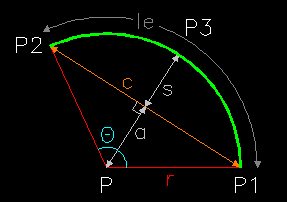
\includegraphics[width=0.5\textwidth]{figures/arcgeom.png}
	\captionof{figure}{Геометрия дуги окружности}
	\label{fig:arcgeom}
\end{figure}

Так как дуга окружности описывает часть этой окружности, то она и обладает всеми атрибутами данной окружности (см. рис. \ref{fig:arcgeom}). Среди них:

\begin{itemize}
	\item Радиус ($r$) --- радиус дуги такой же, как и у окружности;
	\item Центр ($P$) --- тот же, что и у окружности;
	\item Центральный угол ($\Theta$) --- в окружности равен $360^{\circ}$;
	\item Длина дуги ($le$) --- является частью периметра (длины) окружности.
\end{itemize}

Для дальнейшей работы с геометрией дуг примем, также, следующие специфичные атрибуты:

\begin{itemize}
	\item Начальная и конечная точка ($P1, P2$) --- это «вершины» дуги. Хотя иногда и целесообразно говорить о конкретных точках, не лежащих на концах дуги;
	\item Длина хорды ($c$) --- у дуг и окружностей можно провести бесконечное количество хорд, но для нас интерес представляет только хорда, проходящая через её вершины;
	\item Середина дуги ($P3$) --- точка, делящая дуги с данными вершинами на две, равные по длине, дуги;
	\item Апофема ($a$) --- это отрезок, вершинами которого являются середина дуги и её центр. Апофема перпендикулярна хорде;
	\item Высота дуги ($s$) --- это отрезок, проведённый из середины дуги перпендикулярно к хорде.
\end{itemize}

 Кроме самой себя, дуга может, также, и описывать другие геометрические формы: круговой сегмент и сектор. Обе геометрические формы включают в себя все вышеперечисленные атрибуты, однако для выведения формулы параметра \textit{bulge} (выпуклости), потребуется рассмотрение только кругового сектора.

В документации AutoCAD \cite{Autodesk} выпуклостью называется тангенс четверти угла дуги между выбранной вершиной и следующей вершиной в списках вершин полилиний. Отрицательность параметра \textit{bulge} указывает на то, что дуга отрисовывается по часовой стрелке от выбранной вершины к следующей. Выпуклость, равная нулю --- прямой сегмент, выпуклость, равная единице --- половина окружности.

Проблема «расшифровки» атрибутов дуги для дальнейших манипуляций с ней заключается в том, что входными данными являются только координаты вершин и рассматриваемый параметр --- \textit{bulge}.

В самом деле, взяв арктангенс от параметра \textit{bulge} и умножив его на $4$, легко получить центральный угол, на который опирается рассматриваемая дуга. Результат получен в радианах. Для перевода значения в градусы, необходимо умножить это значение на $\pi$ и разделить на $180^{\circ}$.

Для вывода данной зависимости, рассмотрим дугу окружности (см. рис. \ref{fig:arcchord}).

\begin{figure}[H]
	\centering
	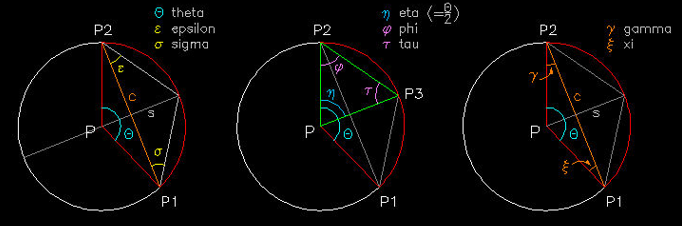
\includegraphics[width=1.0\textwidth]{figures/arcchord.png}
	\captionof{figure}{Дуга окружности с проведённой хордой и углами при ней}
	\label{fig:arcchord}
\end{figure}

Если провести к углу $\Theta$ биссектрису, то получится синий угол $\eta$. В итоге, мы получим равнобедренный треугольник (зеленый), в котором углы $\varphi$ и $\tau$ равны. Поскольку сумма углов в треугольнике всегда равна $180^{\circ}$ градусам, мы теперь знаем, что углы $\varphi$ и $\tau$ равны следующему (\ref{F:phi}):

\begin{equation}
	\varphi=\tau=\frac{(180^{\circ}-\frac{\Theta}{2})}{2}\Rightarrow\varphi=90^{\circ}-\frac{\Theta}{4}
	\label{F:phi}
\end{equation}

Теперь посмотрим на хорду $c$, проведённую от $P1$ до $P2$. Вместе с красными катетами угла $\Theta$ она тоже образует равнобедренный треугольник, а значит, $\gamma=\xi$. Угол при вершине треугольника $P-P1-P2$ --- это центральный угол $\Theta$, поэтому $\gamma$ и $\xi$ вычисляются следующим образом (\ref{F:gamma}):

\begin{equation}
	\gamma=\xi=\frac{180^{\circ}-\Theta}{2}\Rightarrow\gamma=90^{\circ}-\frac{\Theta}{2}
	\label{F:gamma}
\end{equation}

Таким образом, желтый угол $\varepsilon$ должен быть равняться разнице между фиолетовым углом $\varphi$ и оранжевым углом $\gamma$. Другими словами, $\varepsilon$ --- это четверть центрального угла $\Theta$ (\ref{F:epsilon}):

\begin{equation}
	\varepsilon=(90^{\circ}-\frac{\Theta}{4})-(90^{\circ}-\frac{\Theta}{2})\Rightarrow\varepsilon=\frac{\Theta}{2}-\frac{\Theta}{4}=\frac{\Theta}{4}
	\label{F:epsilon}
\end{equation}

Параметр \textit{bulge} (выпуклость) описывает, насколько дуга «выпирает» из вершин, то есть насколько велика высота дуги ($s$) (или расстояние от $P3$ до $P4$). Высота образует катет прямоугольного треугольника с углом, равным четверти центрального угла (см. желтый треугольник $P-P2-P3$ на рис. \ref{fig:epsilon}), и поскольку тангенс описывает отношение между катетами в прямоугольном треугольнике, легко описать геометрию с помощью этого одного угла (\ref{F:epsilon}):

\begin{equation}
	\frac{\sin(\varepsilon)}{\cos(\varepsilon)}=\tan(\varepsilon)
	\label{F:epsilon}
\end{equation}

\begin{figure}[H]
	\centering
	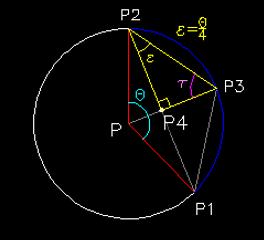
\includegraphics[width=0.5\textwidth]{figures/epsilon.png}
	\captionof{figure}{Связь угла $\varepsilon$ с центральным углом}
	\label{fig:epsilon}
\end{figure}

Мы, также, могли бы найти тангенс угла $\varepsilon$, просто разделив противолежащий катет на смежный катет --- что означает высоту дуги $s$, делённую на половину длины хорды $c$, --- но не зная $s$ и уже имея тангенс $\varepsilon$, полезнее найти $s$ (\ref{F:s}):

\begin{equation}
	s=\frac{c}{2}\cdot\tan(\varepsilon)
	\label{F:s}
\end{equation}

Примем

\begin{equation}
	\tan(\varepsilon)=bulge
	\label{F:tanepsilon}
\end{equation}

Тогда

\begin{equation}
	s=\frac{c}{2}\cdot bulge
	\label{F:sfinal}
\end{equation}

Таким образом, радиус дуги может быть найден следующим образом (\ref{F:r}):

\begin{equation}
	r=\frac{(\frac{c}{2})^2+s^2}{2s}
	\label{F:r}
\end{equation}

Знак той или иной выпуклости важен для определения дуги относительно вершин. Если выпуклость положительна, это означает, что дуга идёт против часовой стрелки от начальной вершины до конечной вершины. Если выпуклость отрицательна, это означает, что дуга идет, наоборот --- по часовой стрелке.

Поэтому все приведенные выше формулы должны касаться абсолютного значения выпуклости, а не фактического значения, иначе можно получить отрицательный радиус.

Итак, поняв, что $bulge = tan(\frac{\Theta}{4})$, в согласовании с документацией AutoCAD \cite{Autodesk} примем, что \textit{bulge} положителен, когда при передвижении от начальной точки дуги к конечной движение происходит против часовой стрелки.

Ясно, что когда $\Theta=0$, то и $bulge(\Theta)=0$. Для углов в $180^{\circ}$ условно принимается, что $bulge(\Theta)=\pm1$. В случае, когда $\Theta=90^{\circ}$, получим следующее (\ref{F:theta90}):

\begin{equation}
	bulge(90^{\circ})= \tan(\frac{90^{\circ}}{4})=\tan(\frac{\pi}{8})
	\label{F:theta90}
\end{equation}

Используя зависимость для тангенса половинного аргумента (\ref{F:tanhalfarg}):

\begin{equation}
	\tan(\frac{\alpha}{2})=\pm\frac{\sin(\frac{\alpha}{2})}{\cos(\frac{\alpha}{2})}=\pm\frac{2\sin^2(\frac{\alpha}{2})}{2\sin(\frac{\alpha}{2})\cos(\frac{\alpha}{2})}=\pm\frac{1-\cos(x)}{\sin(x)}
	\label{F:tanhalfarg}
\end{equation}

Для $\alpha=\frac{\pi}{8}$ получим (\ref{F:bulge90}):

\begin{equation}
	bulge(90^{\circ})=\tan(\frac{\pi}{8})=\pm\frac{1-\cos(\frac{\pi}{4})}{\sin(\frac{\pi}{4})}=\pm\frac{1-\frac{\sqrt2}{2}}{\frac{\sqrt2}{2}}=\pm\frac{1-\frac{1}{\sqrt2}}{\frac{1}{\sqrt2}}=\pm(\sqrt2-1)
	\label{F:bulge90}
\end{equation}



В результате, математические данные совпадают с документацией AutoCAD \cite{Autodesk} и гласят, что

\begin{enumerate}
	\item $bulge = 0$ для отрезка прямой,
	\item $bulge = \pm1$ для дуги в $180^{\circ}$ (половина окружности),
	\item $bulge = \pm(\sqrt2-1) \approx0.41421...$ для четвертей окружностей, когда угол раствора дуги равен $90^{\circ}$.
\end{enumerate}

%%% Local Variables:
%%% mode: latex
%%% TeX-master: "rpz"
%%% End:

\chapter{Разработка программного обеспечения <<DXF Primiview>>}
\label{cha:design}

В данном разделе описывается процесс создания ПП для обработки геометрической информации 2D-объектов специального типа. Обосновывается выбор языка программирования, разрабатываются алгоритмы для разработки ПО, описывается процесс разработки конвертеров.

\section{Выбор языка программирования}

Для написания программы выбран язык программирования Python версии 3.11. Выбор языка программирования обоснован несколькими факторами.

\paragraph{Библиотеки.} Для создания описанного ПП необходимо привлечение различных библиотек. Кроме стандартной библиотеки, с Python можно использовать множество прикладных библиотек, несколько из которых будут описаны в следующих частях работы. Специфичные библиотеки, позволяющие <<читать>> DXF-файл и обрабатывать содержимое внутри него, написаны не для каждого ЯП. Библиотека <<eazy dxf>> для Python позволяет быстро и удобно выполнять данные операции.

\paragraph{Кроссплатформенность.} Большинство программ, написанных на Python, выполняются корректно на всех основных платформах. Перенос программы между операционными системами реализуется простым копированием кода. Кроме того, в процессе разработки ПО, для реализации пользовательского интерфейса используется набор расширений Qt, который тоже работает на таких платформах, как Linux и другие UNIX-подобные ОС, macOS и Windows.

\paragraph{Скорость и удобство разработки.} Удобочитаемсть, ясность и высокое качество этого языка позволяют повысить производительность разработчика во много раз, сравнивая, например, с компилирующими или строго типизированными языками, такими как C, C++ и Java. Объём программного кода на языке Python обычно составляет треть или даже пятую часть эквивалентного программного кода на языке C++ или Java. Кроме того, при запуске программы, написанной на ЯП Python минуются длинные этапы компиляции и связывания, необходимые в некоторых других ЯП, что, также, увеличивает производительность труда программиста \cite{learnpython3}.

\section{Разработка алгоритмов}

Для создания программного обеспечения необходимо сначала разработать концепцию функционирования программы, опираясь на её назначение, на основные её функции. Когда определены модули, блоки и функциональные части ПО, можно приступать к разработке его на выбранном ЯП.

\subsection{Структура программы}

Основываясь на цели, поставленной во введении, разрабатываемая утилита должна принимать на входе DXF-файл, то есть открывать его и обрабатывать его содержимое. Для проверки правильности обработанных данные, то есть, для верификации содержимого DXF-файла, программа должна визуализировать для пользователя обработанное. После верификации обработанных данных и, соответственно, подтверждения соответствия их исходным, пользователю должна предоставляться возможность конвертировать эти данные в какой-либо из предлагаемых форматов. За это отвечает модуль экспорта, который, в свою очередь, подразделяется на четыре модуля, отвечающие за преобразование данных в различные форматы. Среди них следующие:

\begin{enumerate}
	\item Модуль экспорта в TXT-файл, где данные будут представлены в такой же форме, как и в оригинальном DXF-файле, за исключением того, что содержаться в нём будут только поддерживаемые сущности (LINE, POLYLINE, ARC, CIRCLE).
	\item Модуль экспорта в TXT-файл, в котором поддерживаемые сущности будут представлены сочетанием двух строк, первая из которых --- начальная точка примитива, вторая --- конечная. Вторая строка содержит в себе радиус скругления примитива, переходящего из первой точки во вторую.
	\item Модуль экспорта в формат SVG, который, при открытии, векторно отображает информацию в нём.
	\item Модуль экспорта JSON-формат. В данном формате, по подобию формату TXT (x, y, r), содержаться точки, олицетворяющие начало и конец того или иного примитива. В данном случае информация в файле тэгированная, что означает, что в дальнейшем несложно будет получить желаемые куски данных из потенциально объёмного JSON-файла путём обращения по желаемому тэгу.
\end{enumerate}


Схему, отображающую основное содержание разрабатываемого ПО, можно наблюдать на рисунке \ref{fig:organisationsdiagramm}.

\begin{figure}[H]
	\centering
	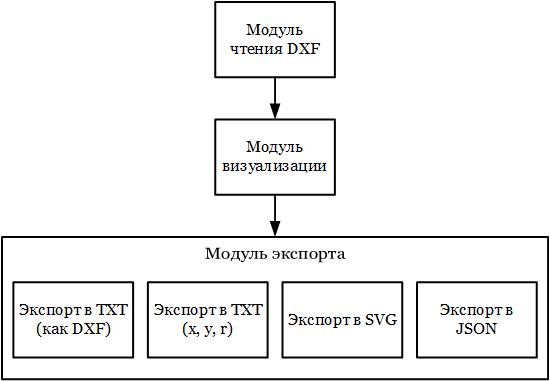
\includegraphics[width=0.8\textwidth]{figures/organisationsdiagramm.png}
	\captionof{figure}{Принципиальная структура ПО <<Primiview>>}
	\label{fig:organisationsdiagramm}
\end{figure}


\subsection{Алгоритмы модулей программы}

В данном пункте приводится описание алгоритмов ПО <<Primiview>> в виде псевдокода.

\paragraph{Алгоритм чтения DXF-файлов.} Алгоритм \ref{alg:readdxf} показывает схему работы процесса извлечения поддерживаемых ПО Primiview примитивов из выбранного DXF-файла.

На первой итерации осуществляется разбиение блоков, в которых могут быть <<спрятаны>> остальные сущности. В случае, если пропустить данный этап, то объекты, находящиеся внутри блоков не будут видны библиотекой \textit{ezdxf}, которая используется для чтения DXF-файлов.

После <<разрушения>> всех блоков примитивы становятся <<видимыми>>. Далее запускается цикл, итерирующий объекты пространства объектов модели (\textit{modelspace}). В случае совпадения объекта с одной из поддерживаемых сущностей, она сохраняется в список соответствующих объектов в оперативной памяти программы. Списком далее будет называться изменяемый упорядоченный тип данных, представляющих собой последовательность элементов, разделённых между собой запятой и заключённых в квадратные скобки. Данный тип данных используется в ЯП Python, поэтому для соблюдения общности, термин будет применяться и в части \ref{sec:software} этого раздела.

Примем ряд условных обозначений:

$msp$ --- пространство объектов модели (modelspace);

$\dashrightarrow$ --- запись объекта в множество.


\begin{algorithm}[H]
	\SetAlgoLined
	\KwData{путь к DXF-файлу}
	\KwResult{массивы примитивов и информации о них в оперативной памяти программы}
	инициализация;
		
	\For{$\forall$ сущн. типа Вставка (INSERT) $\in msp$}{разбиение сущности}
	
	\For{$\forall$ сущн. $\in msp$}{
		\If{сущ явл. линией}{сущн. $\dashrightarrow$ множ. линий}
		\ElseIf{сущн. явл. дугой}{сущн. $\dashrightarrow$ множ. дуг}
		\ElseIf{сущн. явл. окружностью}{сущн. $\dashrightarrow$ множ. окружностей}
		\ElseIf{сущн. явл. полилинией}{сущн. $\dashrightarrow$ множ. полилиний}
	}
	
	\caption[Сохранение поддерживаемых примитивов; из DXF в оперативную память программы]
	{\tabular[t]{@{}l@{}}Сохранение поддерживаемых примитивов \\ из DXF в оперативную память программы\endtabular}
	\label{alg:readdxf}
\end{algorithm}

\paragraph{Алгоритм записи примитивов в TXT (как DXF).} Принцип данного алгоритма (см. алгоритм \ref{alg:dxfintotxt}) основан на открытии созданного TXT-файла, а после --- перебора прочитанных из DXF примитивов и записи из каждого из них необходимой информации в открытый для редактирования TXT-файл.

Записи в текстовом файле должны выглядеть следующим образом (см. листинг \ref{list:txtdxfsicht}):
%\begin{verbatim}
%	LINE(#01)
%	0.1 0.1
%	0.1 0.1
%\end{verbatim}

\begin{lstlisting}[caption={Пример содержания TXT-файла (как DXF)},label=list:txtdxfsicht]
	LINE(#01)
	0.1 0.1
	0.1 0.1
\end{lstlisting}

\begin{algorithm}[H]
	\SetAlgoLined
	\KwData{путь к имя.txt}
	\KwResult{имя.txt (как DXF)}
	инициализация;
	
	\For{$\forall$ LINE $\in$ множ. линий}{записать в файл: атрибут сущности, $x_0, y_0$, $x_1, y_1$; перевести курсор на новую строку}
	
	\For{$\forall$ ARC $\in$ множ. дуг}{записать в файл: атрибут сущности, $x_0, y_0$, $x_1, y_1$, $r$; перевести курсор на новую строку}
	
	\For{$\forall$ CIRCLE $\in$ множ. окруж.}{записать в файл: атрибут сущности, $x_c, y_c$, $r$; перевести курсор на новую строку}
	
	\For{$\forall$ LWPOLYLINE $\in$ множ. полилин.}{записать в файл атрибут сущности;
		
		\For{$\forall$ точки LWPOLYLINE}{
			
			\For{$\forall$ координаты x, y}{записать в файл значение координаты}
			}
		перевести курсор на новую строку}
	\caption{Запись примитивов в TXT (как DXF)}
	\label{alg:dxfintotxt}
\end{algorithm}

В алгоритме \ref{alg:dxfintotxt} $x_0, y_0$ --- координаты начала примитива; $x_1, y_1$ --- координаты конца примитива; $x_c, y_c$ --- координаты центра окружности; $r$ --- радиус дуги или окружности.

\paragraph{Алгоритм записи примитивов в TXT (x,y,r).} Алгоритм \ref{alg:primsintotxt} призван, так же как и в прошлом случае, в открытый только что созданный текстовый файл записать информацию о примитивах, которые были прочитаны из выбранного DXF-файла.

Записи в текстовом файле должны выглядеть следующим образом (см. листинг \ref{list:primsdxfsicht}):
%\begin{verbatim}
%	1.52 1.86 0
%	1.12 2.08 0
%	1.16 2.04 4.0
%	...
%\end{verbatim}

\begin{lstlisting}[caption={Пример содержания TXT-файла (x, y, r)},label=list:primsdxfsicht]
	1.52 1.86 0
	1.12 2.08 0
	1.16 2.04 4.0
	...
\end{lstlisting}

Полилиния может содержать в себе, как отрезки, так и дуги. В объектах LWPOINT сущности LWPOLYLINE степень искривления показывает параметр \textit{bulge}, суть которого подробно описана в разделе \ref{sec:allaboutdxf}. Так как желаемый формат вывода информации о примитивах содержит именно радиус примитива, а не параметр искривления, то необходимо удобно получить радиус из \textit{bulge}.

Для этого воспользуемся уже выведенной зависимостью \cite{ukoloff} и применим её в принятых обозначениях (\ref{F:rad}):

\begin{equation}
	R=|bulge+\frac{1}{bulge}|\cdot\frac{|A-Z|}{4},
	\label{F:rad}
\end{equation}

где A --- начальная точка;

Z --- конечная точка.

Примем, что $A(x_0,y_0), B(x_1,y_1)$. Тогда $AZ(x_1-x_0; y_1-y_0)$.
Таким образом, длина вектора через декартовы координаты (\ref{F:veclen}):
\begin{equation}
	|A-Z|=\sqrt{(x_1-x_0)^2+(y_1-y_0)^2}
	\label{F:veclen}
\end{equation}


\begin{algorithm}[H]
	\SetAlgoLined
	\KwData{текущая точка, следующая точка}
	\KwResult{радиус сегмента полилинии}
	инициализация;
	
	\If{$bulge$ (текущей точки) $=0$}{$r=0$}	
	\Else{$r=|bulge+\frac{1}{bulge}|\cdot\frac{\sqrt{(x_{nexP}-x_{prevP})^2+(y_{nexP}-y_{prevP})^2}}{4}$}
	
	\caption{Вычисление радиуса сегмента полилинии}
	\label{alg:polyarcrad}
\end{algorithm}

Примем условные обозначения:

$\rightsquigarrow$ --- запись в файл;

$newline$ --- перевод на новую строку.

\begin{algorithm}[H]
	\SetAlgoLined	
	\KwData{путь к имя.txt}
	\KwResult{имя.txt (x,y,r)}	
	\ForEach{LINE $\in$ множ. линий}{$x_0 \quad y_0 \quad 0\rightsquigarrow$ имя.txt; \quad $x_1 \quad y_1 \quad 0 \rightsquigarrow$ имя.txt}
	
	\ForEach{ARC $\in$ множ. дуг}{$x_0 \quad y_0 \quad 0\rightsquigarrow$ имя.txt; \quad $x_1 \quad y_1 \quad r \rightsquigarrow$ имя.txt}
	
	\ForEach{CIRCLE $\in$ множ. окруж.}{$x_c + r \quad y_c \quad 0\rightsquigarrow$ имя.txt\tcc*{первая половина окруж.} $x_c - r \quad y_c \quad r \rightsquigarrow$ имя.txt \\  $x_c - r \quad y_c \quad 0 \rightsquigarrow$ имя.txt\tcc*{вторая половина окруж.} $x_c + r \quad y_c \quad r \rightsquigarrow$ имя.txt} \ForEach{POLYLINE $\in$ множ. полилиний \\ prevPoint=None \tcc*{предыдущая точка}}{
		\ForEach{LWPOINT $\in$ множ. точек. полилинии}{
			\If{prevPoint$\neq$None}{r = алгоритм \ref{alg:polyarcrad} (prevPoint, LWPOINT)
			$x(prevP) \quad y(prevP) \quad 0 \rightsquigarrow$ имя.txt\\
			$x(lwpoint) \quad y(lwpoint) \quad r \rightsquigarrow$ имя.txt
			}
		$prevPoint = lwpoint$
		} \newpage
		\If{контур замкнут}{
		r = алгоритм \ref{alg:polyarcrad} (prevPoint, LWPOINT) \\
		$x(lwpoint_\text{посл}) \quad y(lwpoint_\text{посл}) \quad 0 \rightsquigarrow$ имя.txt\\
		$x(lwpoint_\text{перв}) \quad y(lwpoint_\text{перв}) \quad r \rightsquigarrow$ имя.txt
		}
	}
	\caption{Запись примитивов в TXT (x, y, r)}
	\label{alg:primsintotxt}
\end{algorithm}

\paragraph{Алгоритм записи примитивов в SVG.} Формирования файла типа SVG отличается от предыдущих двух, так как этот формат представляет собой язык разметки, а значит, имеет правила синтаксиса, грамматики и т.д. Это расширение языка разметки XML, поэтому в начале, в преамбуле, указывается версия XML, кодировка символов и указание синтаксическому анализатору об игнорировании любых объявлений разметки в определении типа документа.

\begin{lstlisting}[language=XML,caption={Первая строка SVG-файлов},label=list:1stsvgline]
	<?xml version="1.0" encoding="UTF-8" standalone="no"?>
\end{lstlisting}

Следующие две строки должны содержать определение типа документа (заголовок DOCTYPE), однако, данное объявление может оказаться источником ошибок при применении в браузере Mozilla Firefox. Поэтому вместо этого используется атрибут \Code{baseProfile} со значением <<full>> внутри элемента <svg>.

Начиная с четвёртой строки объявляется корневой элемент <svg>:

\begin{lstlisting}[language=XML,caption={Первая строка SVG-файлов},label=list:4thsvgline]
	<svg version="1.1" width="100%" height="100%"
	viewBox="102.1188828597992 -211.7921423734452 50.000000000000014 26.0"
	baseProfile="full"
	xmlns="http://www.w3.org/2000/svg"
	xmlns:xlink="http://www.w3.org/1999/xlink"
	xmlns:ev="http://www.w3.org/2001/xml-events">
\end{lstlisting}

В листинге \ref{list:4thsvgline} присутствует необязательный элемент \Code{viewBox}, который представляет собой параметр с четырьмя значениями, отделяемыми пробелами, определяющими квадратную рамку, в которой будет располагаться графика. Данный атрибут позволяет автоматически масштабировать изображение до размеров указанного контейнера, причём, без потери качества, так как графическая информация храниться и воспроизводится в векторном формате.

Первые два значение --- минимальные координаты $x$ и $y$ рамки, в которой располагается изображение. Третье и четвёртое значения --- соответственно, ширина и высота рамки, в которой находится изображение. Значения указываются в пикселях.

Таким образом, чтобы перенести данные из DXF в SVG, сначала определяются эти четыре значения. Алгоритмы для их определения: алгоритм \ref{alg:allcoords}, алгоритм \ref{alg:extremums} и алгоритм \ref{alg:dimes}.

\begin{algorithm}[H]
	\SetAlgoLined
	\KwData{списки примитивов с параметрами}
	\KwResult{список координат $x$, список координат $y$}
	инициализация; пустой список координат $x$, пустой список координат $y$
	\For{$\forall$ LINE $\in$ множ. линий}{$x_0,x_1\dashrightarrow$ список $x$\\$y_0,y_1\dashrightarrow$ список $y$}
	
	\For{$\forall$ ARC $\in$ множ. дуг}{$(x_c+r),(x_c-r)\dashrightarrow$ список $x$\\$(y_c+r),(y_c+r)\dashrightarrow$ список $y$}
	
	\For{$\forall$ CIRCLE $\in$ множ. окруж.}{$(x_c+r),(x_c-r)\dashrightarrow$ список $x$\\$(y_c+r),(y_c+r)\dashrightarrow$ список $y$}
	
	\For{$\forall$ LWPOLYLINE $\in$ множ. полилин.}{
		\For{$\forall$точки в множ. LWPOINTS}{
		$x\dashrightarrow$ список $x$\\$y\dashrightarrow$ список $y$}}
	вернуть список координат $x$ и список координат $y$
	\caption{Вычленение координат изображения из DXF в отдельные списки}
	\label{alg:allcoords}
\end{algorithm}

\begin{algorithm}[H]
	\SetAlgoLined
	\KwData{список координат $x$, список координат $y$}
	\KwResult{$x_{MIN}, y_{MIN}$}
	инициализация;\\
	использовать алгоритм \ref{alg:allcoords}\\
	вернуть $x_{MIN}, y_{MIN}$ из списков стандартными функциями сортировки ЯП
	\caption{Поиск наименьших координат изображения из DXF}
	\label{alg:extremums}
\end{algorithm}

\begin{algorithm}[H]
	\SetAlgoLined
	\KwData{список координат $x$, список координат $y$}
	\KwResult{ширина и высота рамки изображения}
	инициализация;
	использовать алгоритм \ref{alg:allcoords}\\
	определить $x_{MIN}, x_{MAX}, y_{MIN}, y_{MAX}$ из списков стандартными функциями сортировки ЯП\\
	ширина $=x_{MAX}-x_{MIN}$\\
	высота $=y_{MAX}-y_{MIN}$\\
	вернуть значения ширины и высоты
	\caption{Поиск длины и высоты изображения из DXF}
	\label{alg:dimes}
\end{algorithm}





\section{Разработка программного обеспечения}\label{sec:software}


%%% Local Variables:
%%% mode: latex
%%% TeX-master: "rpz"
%%% End:

\chapter{Экономическая часть}
\label{cha:economy}

В данном разделе описаны экономические аспекты проекта по созданию ПО <<Primiview>> для обработки геометрической информации 2D-объектов специального типа.

\section{Экономическое обоснование}

Целью экономического обоснования проекта является представление разработанного ПП в качестве проекта для реализации на предприятии, что позволит провести планирование и корректировку последовательности работ (при необходимости).

\subsection{Разработка проекта}

\paragraph{Цель проекта} --- создание модуля конвертации форматов, как отдельного ПП, для внедрения в ПО для автоматизации технологического проектирования обработки деталей типа <<Втулка>> на станках с ЧПУ к 05.06.2023.

\textit{Обоснование цели}. Клиент --- это производитель станков с ЧПУ. Для создания УП на продаваемые станках клиенты заказчика привлекают САПР, разработанные за рубежом, что негативно влияет на независимость от сторонних организаций, ограниченность в дополнении ПО функционалом, необходимым только на отдельном предприятии, а также, на сохранность информации, используемой при разработке УП. Компания работает над проектом разработки своей CAM-системы для предложения своим клиентам специализированного ПО вместе с оборудованием с целью решить вышеуказанные проблемы. 

Численные критерии сравнения состояний системы клиента:
\begin{itemize}
	\item сложность проектирования,
	\item сроки (время) проектирования,
	\item себестоимость проектирования,
	\item качество результатов проектирования.
\end{itemize}

\textit{Пояснения к критериям}. Под сложностью проектирования понимается минимально-необходимая квалификация проектировщика для выполнения задач технологического проектирования.

Трудоёмкость проектирования, в данном случае, выражается в среднем времени создания (написания) одной УП.

Себестоимость проектирования оценивается не в расчёте на одну УП, а в рамках одного рабочего года. В себестоимость проектирования входят такие элементы, как зарплата сотрудника, производящего проектирование, а также, цена годовой лицензии/контракта обслуживания CAM-системы для данного количества оборудования на предприятии.

В качестве численного критерия для оценки качества результатов проектирования принято среднее количество типов ошибок, корректировки по которым оператор станка с ЧПУ вносит после того, как автоматизированное проектирование выполнено.

\textbf{Текущее состояние системы клиента}: основное ПО по автоматизации технологического проектирования введено в эксплуатацию, базовые потребности системы по конвертации DXF-файлов работают.

По численным критериям:
\begin{itemize}
	\item сложность проектирования: инженер-технолог II категории по квалификационному справочнику \cite{qualification},
	\item сроки (время) проектирования: 3 часа,
	\item себестоимость проектирования: 1420000 руб. (см. раздел \ref{par:ecocalc}),
	\item качество результатов проектирования: 10 ошибок.
\end{itemize}

\textbf{Целевое состояние системы клиента}: усовершенствованная, более гибкая и универсальная версия этого ПО.

По численным критериям:
\begin{itemize}
	\item сложность проектирования: инженер-технолог (без категории) по квалификационному справочнику \cite{qualification},
	\item сроки (время) проектирования: максимум 1,5 часа,
	\item себестоимость проектирования: максимум 1 млн.руб.,
	\item качество результатов проектирования: максимум 5 типов ошибок.
\end{itemize}

\textbf{Результатом} проекта является созданные и готовый к работе ПП, на вход которому подаётся DXF и информация о поддерживаемых примитивов в котором конвертируется в файлы форматов TXT, SVG и JSON. Файлы последних форматов содержат в себе геометрическое описание объектов по правилам, описанным в предыдущих разделах ВКР, из входного DXF, удобное для дальнейшей работы в CAM-системе "ТокКТЭ".

Команда проекта сформирована из 3 человек, среди которых:
\begin{enumerate}
	\item 1 владелец,
	\item 2 программиста, среди которых:
	\begin{enumerate}
		\item[б.1)] 1 разработчик,
		\item[б.2)] 1 тестировщик.
	\end{enumerate}
\end{enumerate}

Владелец проекта организует работу остальной команды, проводит планирование проекта, оценку его экономической эффективности, контроль за выполнением подчинёнными задач проекта.

Программисты занимаются непосредственно созданием продукта проекта, то есть написанием ПО. Разработчики отвечают за написание программного кода по техническому заданию проекта. Тестировщики выполняют проверку работоспособности ПП, ищут и сообщают отделу разработчиков о найденных и необходимых к устранению ошибок и недочётов программы.




\subsection{Дерево задач проекта}

Целью данного этапа является построение иерархического дерева, включающего в себя последовательное разбиение общей цели проекта на подцели и задачи.

\paragraph{Первый уровень иерархии.}

Главной целью проекта, как уже было сказано, является разработка программного обеспечения <<Primiview>> по конвертации файлов в формате DXF в форматы TXT, SVG, JSON. Данная цель в проекте единственная и находится на высшем уровне иерархии.

\paragraph{Второй уровень иерархии.}

В целях определения и формализации цели, структуры и методов проекта, чтобы исключить неоднозначное их понимание и толкование исполнителями, первый этап, стоящий в иерархии на втором уровне, --- это \textit{формирование технического задания (ТЗ)}.

При параллельном методе разработке, когда этапы проекта могут начинаться тогда, пока предыдущие ещё не закончились, следующим шагом данного уровня будет \textit{разработка алгоритмов} программного обеспечения. Данный этап необходим, так как именно на нём ещё можно решить несостыковки в логической части программы, исправление которых на следующих этапах редко бывает возможным.

Параллельно с разработкой алгоритмов начинается этап непосредственно \textit{разработки ПО}. Эти этапе происходят одновременно, так как они тесно взаимосвязаны, и, например, не зная на каком ЯП будет разрабатываться ПО, трудно будет рационально подобрать алгоритмы, отвечающие возможностям ЯП.

Завершающим этапом второго уровня является \textit{сдача проекта} заказчику. Эта стадия может быть выполнена только при полном выполнении предыдущих стадий, если иное не было предварительно оговорено с заказчиком.

\paragraph{Третий уровень иерархии.}

Этап формирования ТЗ подразделяется на следующие задачи:

\begin{enumerate}
	\item Определение назначения ПО. Здесь формализуются цели и функции ПП. Впоследующем, они вносятся в ТЗ. Это смысл выполнения проекта, то, к чему стремится вся его команда, что хочет получить в итоге заказчик;
	\item Исследование степени разработанности. На стадии предпроектного исследования выполняется проверка, существуют ли аналоги данного продукта в открытом доступе рынка. Если есть, то чем заказчика не устраивает их использование;
	\item Требования к продукту. Определяются численные критерии, которым должен соответствовать результат проекта на этапе его сдачи;
	\item Определение сроков. Всем участникам проекта необходимо знать, к какому сроку они должны выполнить определённый ранее объём работ. Сотрудникам, при согласовании ТЗ, необходимо оценить эти сроки, и в случае невозможности из соблюдения, просить корректировки и согласования с заказчиком более позднего выполнения задач;
	\item Написание ТЗ. Завершающая стадия этапа формирования ТЗ --- здесь собирается вся информация с предыдущих стадий и документируется согласно стандартам организации. ТЗ должно быть согласовано со всему участниками проекта.
\end{enumerate}

Этап разработки алгоритмов подразделяется на следующие стадии:
\begin{enumerate}
	\item Определение принципа работы ПО. Составляется принципиальная схема работы ПО, связь модулей, определяется предназначение каждого из модулей;
	\item Разработка алгоритмов для модулей ПП. Происходит решение поставленных задач на уровне логики и математики, строится набор взаимосвязей алгоритмов. По возможности, рассматривается применение уже существующих универсальных (реже, специальный) алгоритмов.
\end{enumerate}

Этап разработки ПО содержит такие стадии:
\begin{enumerate}
	\item Выбор ЯП. Данная стадия подразумевает проведение сравнительного анализа существующих инструментов различных ЯП применительно к разрабатываемому ПП;
	\item Определение структуры ПО. Эта стадия необходима для понимания разработчика функционала каждого из модулей программы. От этого зависит, на какие части (из каких файлов) будет состоять ПО;
	\item Написание и отладка программного кода. Главная часть создания продукта. На этой стадии разработчики непосредственно пишут программный код и отлаживают его работу.
	\item Тестирование ПО. Команда тестировщиков, также, пишет тестовый код, который проверяет разрабатываемое ПО на корректность работы его функционала.
\end{enumerate}

Завершающий этап на втором уровне иерархии --- сдача ПО, содержит следующие стадии:
\begin{enumerate}
	\item Презентация. Команда проекта презентует результаты своей работы заказчику, демонстрирует работу программы. Отчитывается по выполнению всех этапов, указанных в ТЗ;
	\item Внесение правок. По итогам презентации команда проекта заслушивает обратную связь от заказчика и на этой основе вносит в проект правки;
	\item Передача ПО заказчику. Организатор проекта передаёт заказчику исходный код ПО, документацию и инструкции, требования, прочие исходные файлы, информацию, обеспечивающую доступ к ПП;
	\item Обучение Сотрудников. При сдаче нового ПП, команде разработчиков необходимо обучить персонал заказчика работе с новым ПО;
	\item Устранение недостатков. После обучения исполнитель проекта (организация) предоставляет заказчику 7 рабочих дней на проведение внутренних проверок ПО, по результатам которых заказчик предоставляет исполнителю список исправлений, которые команда проекта обязана скорректировать в разработанном ПО;
	\item Закрытие задания на проект. Расчёт. Конечным мероприятием сдачи ПО являет закрытие сторонами задания по договору и получение расчёта за выполненную работую.
\end{enumerate}

\paragraph{Четвёртый уровень иерархии.}

Описание данного уровня иерархии приведено кратко для примера. В самом деле, каждая из стадий третьего уровня подразделяется на задачи четвёртого уровня.

Стадия исследования степени разработанности проблемы в этапе формирования ТЗ подразделяется на следующие задачи:
\begin{enumerate}
	\item Исследование отечественного рынка аналогичных ПП. Задача состоит в поиске решений по аналогичным проектам в открытом доступе в рамках отчественного рынка;
	\item Исследование зарубежного рынка аналогичных ПП. Данная задача отличается от предыдущей сложностью поиска аналогов (на зарубежном рынке(пространстве)), так как для проведения данного анализа необходим высокий уровень владения иностранным (английским) языком, а также, требуется знание достоверных ресурсов (источников) информации.
\end{enumerate}

Описанные элементы иерархии сведены в иерархическое дерево (см. рисунок \ref{fig:projektaufgaben}). Уровни иерархической структуры оформлены таким образом, что, чем конкретнее описаны элементы структуры, тем насыщеннее цвет заливки.

	
\begin{figure}[H]
	\centering
	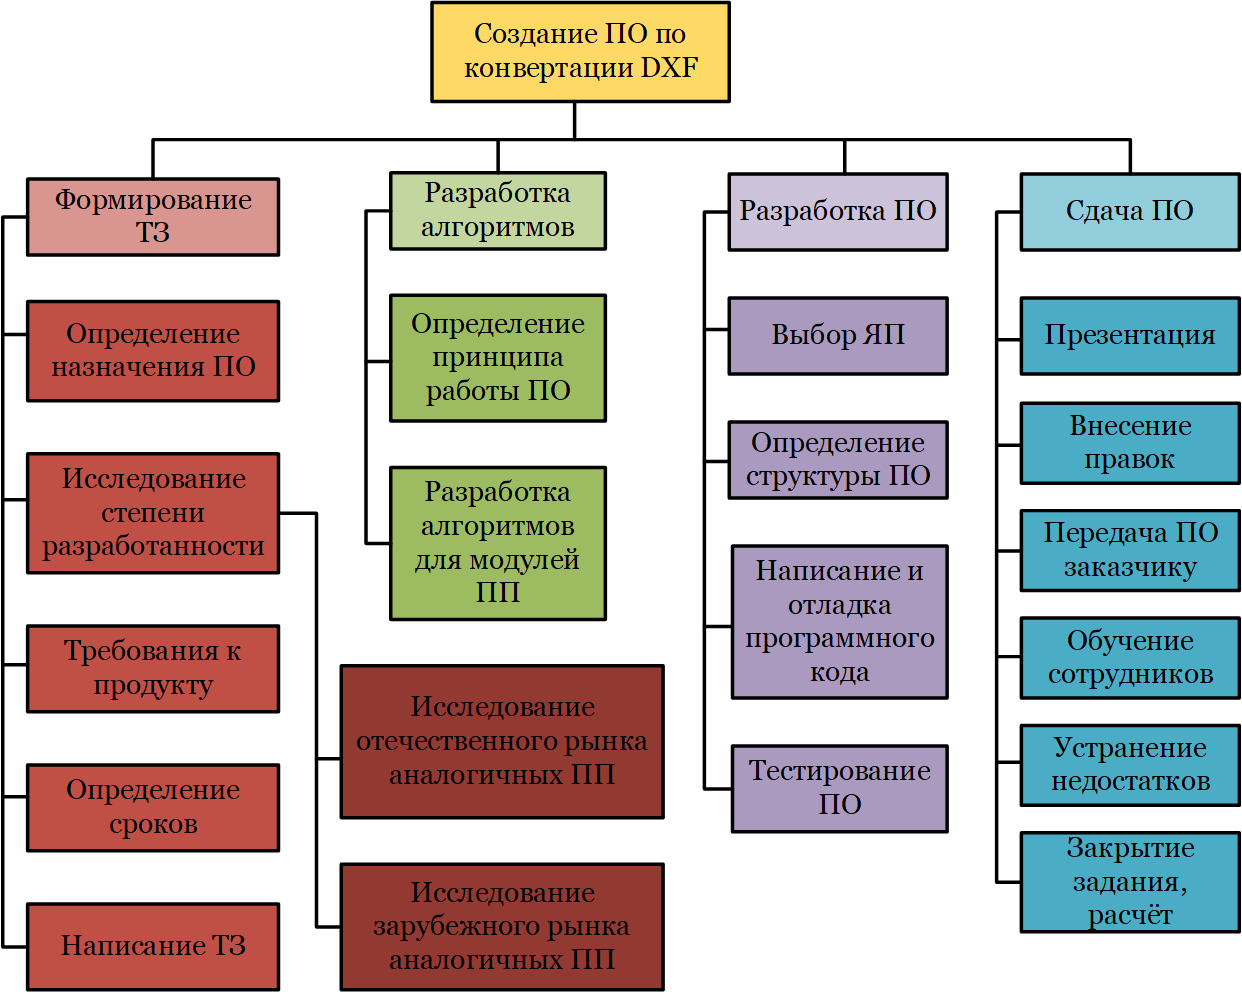
\includegraphics[width=1.0\textwidth]{figures/projektaufgaben.png}
	\captionof{figure}{Дерево задач проекта}
	\label{fig:projektaufgaben}
\end{figure}

\subsection{Построение диаграмм проекта}

На данном этапе строится диаграмма Ганта (англ. Gantt Chart, также, ленточная диаграмма, график Ганта) --- это тип столбчатых диаграмм, использующийся для иллюстрации плана, графика работ проекта. Также, является методом планирования проекта. Эта диаграмма представляет собой отрезки (графические плашки), размещающиеся на горизонтальной шкале времени. Каждый отрезок соответствует отдельно задаче (подзадаче). Начало, конец и длина отрезка на шкале времени соответствуют началу, концу и длительности задачи. Диаграмма может использоваться для представления текущего состояния выполнения работ: часть прямоугольника, отвечающего задаче, заштриховывается, отмечая процент выполнения задачи; показывается вертикальная линия, отвечающая моменту «сегодня».

Рядом с самой диаграммой располагается таблица со списком работ, строки которой соответствуют отдельным задачам, отображённым на диаграмме, в то время как столбцы содержат дополнительную информацию о задаче.


%\begin{sidewaysfigure}[H]
%	\centering
%	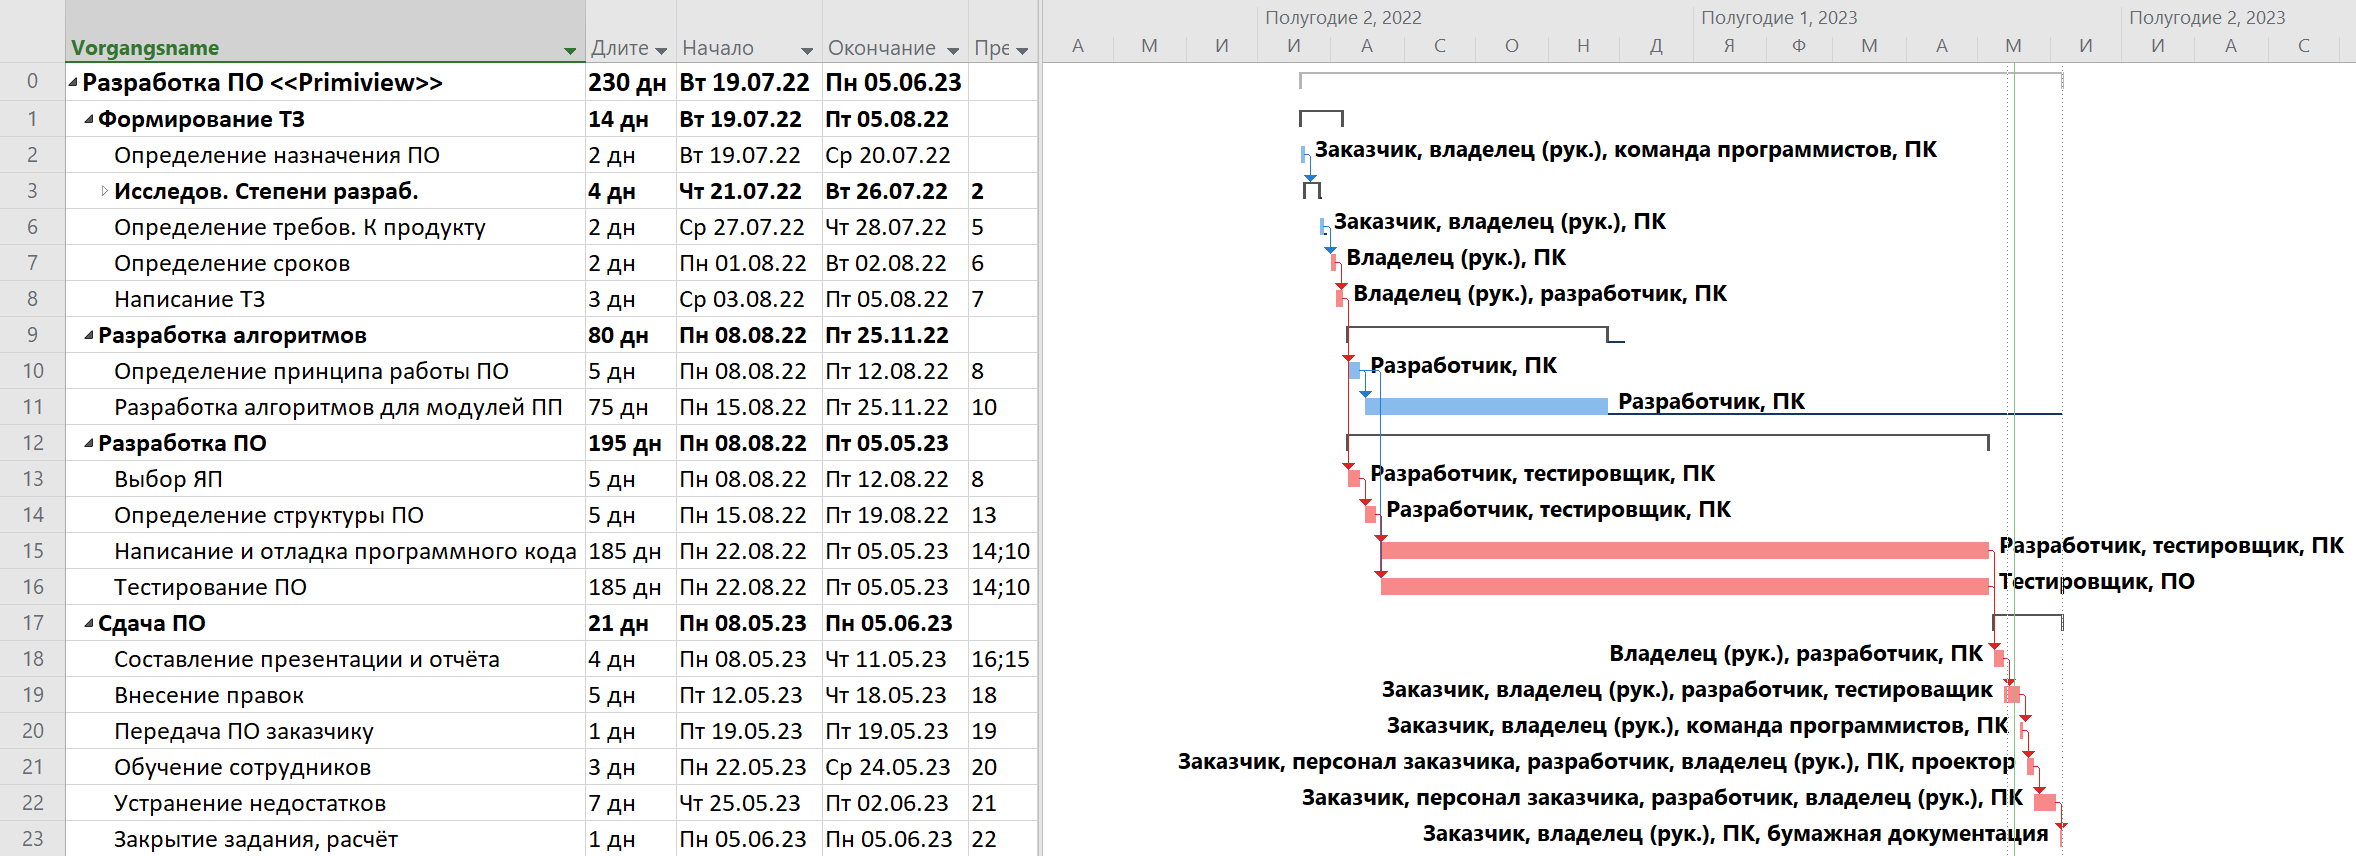
\includegraphics[width=\textwidth, height=0.5\textheight]{figures/gantt.png}
%	\captionof{figure}{Диаграмма Ганта для проекта}
%	\label{fig:gantt}
%\end{sidewaysfigure}


%\begin{landscape}
%\begin{sideways}
%\KOMAoptions{paper=landscape, pagesize}
%\recalctypearea
%\begin{landscape}
\begin{figure}[H]
	\centering
	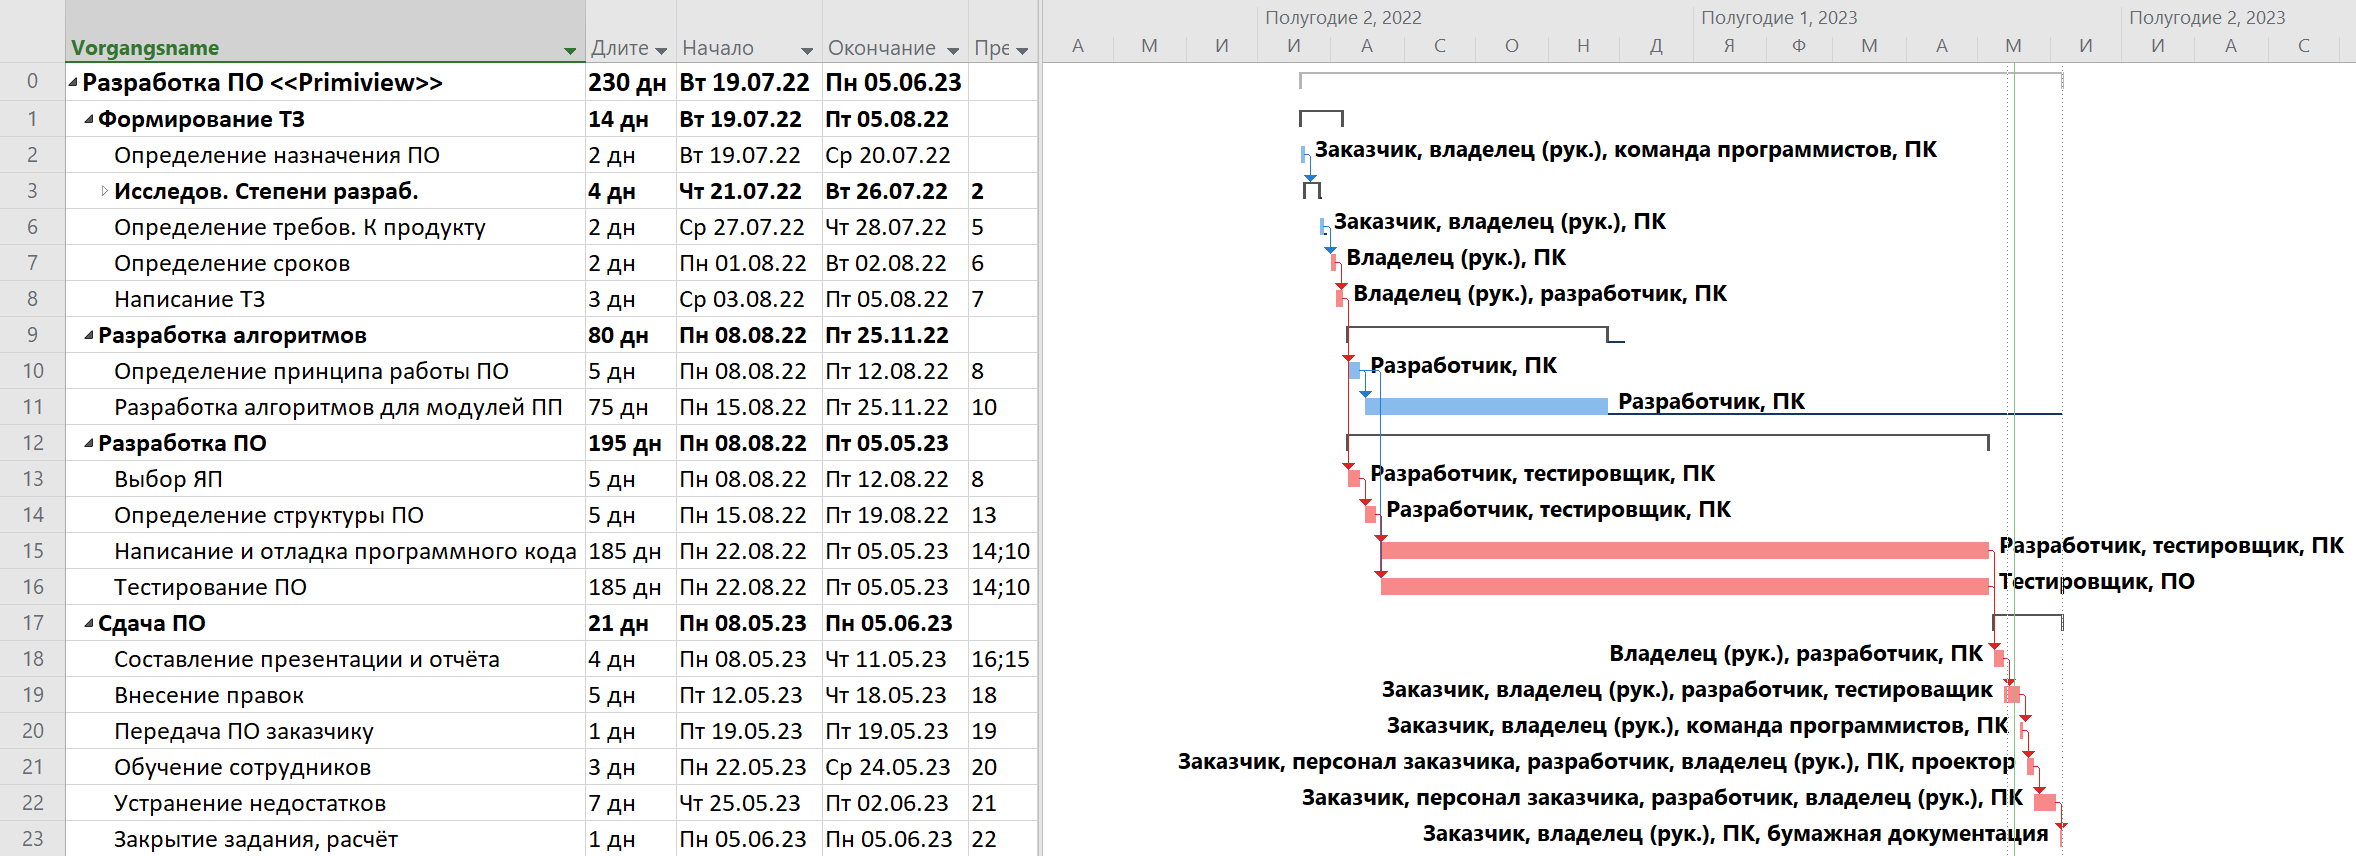
\includegraphics[width=1.4\textwidth, angle=90]{figures/gantt.png}
	\captionof{figure}{Диаграмма Ганта для проекта}
	\label{fig:gantt}
\end{figure}
%\end{landscape}
%\KOMAoptions{paper=portrait, pagesize}
%\recalctypearea
%\end{sideways}
%\end{landscape}


















\section{Сравнительная экономическая эффективность}

Расчеты сравнительной экономической эффективности капитальных вложений (инвестиций) применяются при сопоставлении нескольких возможных для осуществления вариантов инженерных решений: при решении задач по выбору взаимозаменяемых материалов, внедрению новых видов техники, модернизации оборудования, способов организации производственных процессов и т. п. То есть для оценки решений, которые являются альтернативными для обеспечения одинаковых конечных результатов деятельности. При этом конечные результаты (производство конкретной продукции с определенными характеристиками в заданном объеме) уже известны, есть необходимость определить, какой способ ее изготовления на том или ином этапе деятельности предприятия является более выгодным.

\subsection{Исходные данные}

Станкостроительное предприятие рассматривает заказ на создание программного обеспечения для своего оборудования (токарных станков с ЧПУ). Это ПО автоматизирует процесс создания управляющих программ для станков с ЧПУ, взамен работе инженера-технолога-программиста, который, обычно, берёт чертёж детали и либо вручную пишет УП, либо использует иностранные CAM-системы, предварительно создавая 3d-модель по выданному чертежу.
В рамках данной (третьей) части ВКР будет рассматриваться инвестиционный проект (ИП) с точки зрения покупателя оборудования у предприятия, которое привлекло силы университета для создания описанного ПО. Сравниваются два варианта – покупка станков без ПО и, соответственно, с ним.

\paragraph{Сравнительная характеристика вариантов.} Рассмотрим ситуацию с точки зрения покупателя оборудования рассматриваемого станкостроительного предприятия. Соберём основные данные в таблицу  \ref{tab:startcomparis}.

\begin{longtable}{|p{0.50\textwidth}|p{0.50\textwidth}|}%{|p{0.40\textwidth}|c|}
	\caption{Сравнительная характеристика вариантов ИП}
	\label{tab:startcomparis}
	\centering
	\tabularnewline
	\hline
	Вариант 1      & Вариант 2\\
	\hline \endfirsthead
	\subcaption{Продолжение таблицы~\ref{tab:startcomparis}}\\
	\hline \endhead
	\subcaption{Продолжение на след. стр.}
	\endfoot
	%\hline
	\endlastfoot
	Покупка станка без ПО	&	Покупка станка вместе с ПО (CAM-системой) за большую цену\\
	\hline
	Наём во время этапа подготовки производства инженеров-технологов-программистов для написания УП	&	Привлекаются технологи из имеющегося штата сотрудников для выполнения дополнительных обязанностей по контролю создания УП с помощью купленного ПО\\
	\hline
	Время написания УП в три раза дольше, чем во втором варианте	&	Время написания УП в течение одного часа (в среднем)\\
	\hline
\end{longtable}

Варианты рассматриваются с точки зрения потребителя оборудования.
За сопоставляемые характеристики принимаются следующие:

\begin{itemize}
	\item Объём производства (серийное),
	\item Частота создания УП в год (200 новых УП в среднем).
\end{itemize}

\paragraph{Выбор единичного периода времени.} В качестве единичного периода времени для расчётов примем один год, так как на рассматриваемом предприятии-клиенте ситуация с производством каждый месяц практически не меняется. Также, большинство справочных величин ссылаются именно на годовой период, что тоже является подтверждением равномерной распределённости экономических характеристик внутри отдельно взятых месяцев.

\paragraph{Состав и описание капитальных вложений по вариантам.} В капитальные вложения входят следующие величины:

\begin{itemize}
	\item Цена станка с без ПО – 2 750 000 руб.,
	\item Цена встроенной CAM-системы на единицу оборудования– 70 000 руб.,
	\item Наладка полной группы станков – 20 000 руб.
\end{itemize}

\paragraph{Принятие решения по нормативному сроку окупаемости и его обоснование.} Соответствует требованиям к сроку окупаемости дополнительных капитальных вложений, в данном случае – в токарный станок с ЧПУ.

Срок полезного использования оборудования – 10 лет.

Срок контракта на выпуск продукции с использованием данного оборудования – в рассматриваемой ситуации нет ограничений, токарная обработка постоянно проводится на предприятии.

Требования собственника, инвестора – предприятие установило желаемый срок окупаемости – 5 лет.

Следовательно, задаём Тн (нормативный срок окупаемости) равным 5 лет, так как временные рамки требований инвестора меньше срока полезного использования оборудования.

\paragraph{Определение состава затрат по вариантам (результат – перечень затрат).} Корректировка затрат в соответствии с возможностями Методики сравнительной эффективности (включаем в расчет только различающиеся по альтернативам затраты). Деление затрат на переменные и постоянные. Формирование списка исходных данных для выполнения расчетов (см. таблицу \ref{tab:gegeben}).

\begin{longtable}{|p{0.30\textwidth}|p{0.30\textwidth}|p{0.30\textwidth}|}
	\caption{Исходные данные для расчётов текущих затрат}
	\label{tab:gegeben}
	\centering
	\tabularnewline
	\hline
 	\quad & \multicolumn{1}{c|}{Вариант 1} & \multicolumn{1}{c|}{Вариант 2}\\
	\hline \endfirsthead
	\subcaption{Продолжение таблицы~\ref{tab:gegeben}}
	\\ \hline \endhead
	\subcaption{Продолжение на след. стр.}
	\endfoot
	%\hline
	\endlastfoot
	\multicolumn{3}{|c|}{Переменные затраты (на единицу объема деятельности (одну УП))}\\
	\hline
	Зарплата технолога, руб & \multicolumn{1}{c|}{1500} & \multicolumn{1}{c|}{1500}\\
	\hline
	Время на написание одной УП, час & \multicolumn{1}{c|}{3} & \multicolumn{1}{c|}{1}\\
	\hline
	\multicolumn{3}{|c|}{Постоянные затраты (на единицу оборудования)}\\
	\hline
	Цена годовой лицензии/контракта обслуживания CAM-системы, руб & \multicolumn{1}{c|}{50000} & \multicolumn{1}{c|}{55000}\\
	\hline
\end{longtable}

\subsection{Расчёты и анализ}

Так как выбран нормативный срок окупаемости, равный одному году, то к нему будут приведены расчёты по приведённым затратам.

\paragraph{Исходные данные.}

Среднее годовое количество УП на предприятии-покупателе станков
\[N=200 \text{ шт;}\]

Срок полезного использования оборудования:
\[T_{machinery}=10 \text{ лет;}\]

Требования инвестора по окупаемости ИП:
\[T_{inv}=5 \text{ лет;}\]

Принятая норма окупаемости:
\[{T_n=T}_{inv}=5 \text{ лет;}\]

Наладка полной группы станков:
\[{CAM}_{Term}=20000 \text{ руб;}\]

Цена встроенной CAM-системы на единицу оборудования:
\[{CAM}_2=70000 \text{ руб;}\]

Цена станка без встроенной CAM-системы:
\[M=2750000 \text{ руб;}\]

Цена годовой лицензии/контракта обслуживания CAM-системы на единицу оборудования для вариантов 1 и 2, соответственно:
\[{CAM}_{1Perm}=50000 \text{ руб;}\]

\[{CAM}_{2Perm}=55000 \text{ руб;}\]

Среднее время написания одной УП:
\[t_1=3 \text{ часа;}\]
\[t_2=1 \text{ час;}\]

Почасовая оплата технолога:
\[Sal=1500 \text{ руб;}\]

Страховые сбора от заработной платы:
\[fees=30\%\]

Количество покупаемых станков:
\[N_M=5 \text{ шт;}\]

\paragraph{Расчёт.}\label{par:ecocalc}

Себестоимость использования оборудования и ПО:
\begin{equation}
	\begin{aligned}
		C_1 = Sal \cdot t_1\cdot N \cdot(100\%+fees)+N_M \cdot CAM_{1Perm} =\\= 1500 \cdot 3 \cdot 200 \cdot (100\%+30\%)+5 \cdot 50000=1 420 000 \text{ руб;}
	\end{aligned}
\end{equation}
\begin{equation}
	\begin{aligned}
		C_2 = Sal \cdot t_2\cdot N \cdot(100\%+fees)+N_M \cdot CAM_{2Perm} =\\= 1500 \cdot 1 \cdot 200 \cdot (100\%+30\%)+5 \cdot 55000=665 000 \text{ руб;}
	\end{aligned}
\end{equation}

Условно-годовая экономия (на себестоимости):
\begin{equation}
	\begin{aligned}
		E=|C_1-C_2|=|1420000-665000|=755 000 \text{ руб;}
	\end{aligned}
\end{equation}

Капитальные вложения предприятия-покупателя станков:
\begin{equation}
	\begin{aligned}
		K_1=M \cdot N_M+{CAM}_{Term}=2750000 \cdot 5+20000=13 770 000 \text{ руб;}
	\end{aligned}
\end{equation}
\begin{equation}
	\begin{aligned}
		K_2=N_M \cdot (M+{CAM}_2)+{CAM}_{Term}=\\=5 \cdot (2750000+70000)+20000 = 14 120 000 \text{ руб;}
	\end{aligned}
\end{equation}

Дополнительные капитальные вложения:
\begin{equation}
	\begin{aligned}
		K_{extr}=|K_1-K_2|=|13770000-14120000|=350 000 \text{ руб;}
	\end{aligned}
\end{equation}
\begin{equation}
	\begin{aligned}
		K_{extr}=N_M \cdot {CAM}_2=5 \cdot 70000=350 000 \text{ руб. (проверка);}
	\end{aligned}
\end{equation}

Срок окупаемости дополнительных капитальных вложений:
\begin{equation}
	\begin{aligned}
		T_{payback}=\frac{K_{extr}}{E}=\frac{350000}{755000}=0,464 \text{ лет;}
	\end{aligned}
\end{equation}

Приведённые затраты по вариантам:
\begin{equation}
	\begin{aligned}
		Z_1=C_1+\frac{1}{T_n} \cdot K_1=1420000+\frac{1}{5} \cdot 13770000=4 174 000 \text{ руб;}
	\end{aligned}
	\label{F:spends1}
\end{equation}
\begin{equation}
	\begin{aligned}
		Z_2=C_2+\frac{1}{T_n} \cdot K_2=665000+\frac{1}{5} \cdot 14120000=3489000 \text{ руб;}
	\end{aligned}
	\label{F:spends2}
\end{equation}

Годовой экономический эффект:
\begin{equation}
	\begin{aligned}
		E_{annual}=|Z_1-Z_2|=|4174000-34890000|=685000 \text{ руб;}
	\end{aligned}
\end{equation}

Минимальный годовой объём деятельности, при котором обеспечивается приведённый годовой экономический эффект:
\begin{equation}
	\begin{aligned}
		N_{cr}=\frac{N_M \cdot CAM_{1Perm}-N_M \cdot CAM_{2Perm}-\frac{K_{extr}}{T_n}}{S \cdot t_2 \cdot (100\%+fees)-Sal \cdot t_1 \cdot (100\%+fees)}=\\=\frac{5 \cdot 50000-5 \cdot 55000-\frac{350000}{5}}{1500 \cdot 1 \cdot 100\%+30\%-1500 \cdot 3 \cdot 100\%+30\%}=24,359 \text{ шт;}
	\end{aligned}
\end{equation}

По вычисленным в формулах \ref{F:spends1}, \ref{F:spends2} затратам изобразим на графике (см. рисунок \ref{fig:economyborders}) границы целесообразности рассматриваемых вариантов.

\pgfplotsset{width=13cm,compat=1.9}
\begin{figure}[H]
	\centering
	\begin{tikzpicture}
		\centering
		\begin{axis}[ 
			xlabel = {$N, \text{шт. (объём деятельности)}$},
			ylabel = {$Z, \text{руб. (приведённые затраты)}$},
			xmin=0, xmax=200, ymin=2900000,
			xtick={0,20,40,60,80,100,120,140,160,180,200},
			ymajorgrids=true,
			xmajorgrids=true
			]
			\addplot[line width=1mm,  blue, mark=*] coordinates {
				(0,3004000) (200,4174000)
			};
			\addplot[line width=1mm,  red, mark=triangle] coordinates {
				(0,3099000) (200,3489000)
			};
%			\node at (axis cs:0,4200000) [anchor = north west] {\text{Границы целесообразности}};
		\end{axis}
		\label{graph:economyborders}
	\end{tikzpicture}
	\captionof{figure}{Границы целесообразности рассматриваемых вариантов}
	\label{fig:economyborders}
\end{figure}

Получив необходимые значения по критериям сравнения, сведём результаты в таблицу \ref{tab:fintabeco}).

%\begin{longtable}{|p{0.40\textwidth}|p{0.05\textwidth}|p{0.15\textwidth}|p{0.15\textwidth}|p{0.15\textwidth}|}
\begin{longtable}{|p{0.40\textwidth}|p{0.05\textwidth}|p{0.13\textwidth}|p{0.13\textwidth}|p{0.13\textwidth}|}
	\caption{Сравнительная характеристика рассматриваемых вариантов по показателям эффективности}
	\label{tab:fintabeco}
	\centering
	\tabularnewline
	\hline
	\multicolumn{1}{|c|}{\multirow{3}{6cm}{Наименование показателя}} & \multicolumn{1}{c|}{\multirow{3}{1cm}{Ед. изм.}} & \multicolumn{2}{c|}{По вариантам:} & \multicolumn{1}{c|}{\multirow{3}{3cm}{Отклонения показателей}}\\
	\cline{3-4} 
	\endfirsthead
	\subcaption{Продолжение таблицы~\ref{tab:fintabeco}}
	\\ \hline \endhead
	\subcaption{Продолжение на след. стр.}
	\endfoot
	%\hline
	\endlastfoot
	\multicolumn{1}{|c|}{}&\multicolumn{1}{c|}{}&Вариант без ПО&Вариант c ПО&\multicolumn{1}{c|}{}\\
	\hline
	Годовой объем деятельности&шт.&200&200&-\\
	\hline
	Капитальные вложения, всего&руб.&13770000&14120000&350000\\
	\hline
	\multicolumn{5}{|l|}{в том числе:}\\
	\hline
	Наладка станков&руб.&20000&20000&-\\
	\hline
	Цена станка (Вар. 2 + ПО)&руб.&13750000&665000&755000\\
	\hline
	Срок окупаемости дополнительных кап. вложений&&0,464&&\\
	\hline
	Приведённые затраты по вариантам&руб.&4174000&3489000&658000\\
	\hline
	Годовой экономический эффект&&&685000&\\
	\hline
\end{longtable}


\subsection{Выводы по результатам расчётов.}

Так как на первых этапах расчёта по методу сравнительной эффективности ИП нельзя было сделать конкретный вывод по поводу целесообразности одного из предлагаемых вариантов по причине того, что по первому варианту себестоимость ИП была больше в сравнении со вторым, а капитальные вложения, соответственно, меньше, то расчёт был продолжен до момента вычисления расчётного срока окупаемости дополнительных капитальных вложений, а также расчёта приведённых затрат по каждому из вариантов.

Исходя из расчётов и построенного по ним графика, сделаем вывод, что, производя уже 25 УП за год, выгоднее становится вариант с ПО, так как приведённые затраты для соответствующего количество производимых УП для этого варианта оказываются меньше.

Анализируя итоговые данные, выбираем для реализации второй вариант, то есть покупка оборудования вместе со встроенным ПО (CAM-системой), объясняя выбор тем, что расчётный срок окупаемости оказался намного меньше рассматриваемого нормативного срока окупаемости (0,4 и 5 лет, соответственно), а приведённые затраты по первому варианту оказались больше, чем по второму.

Действительно, экономия времени на создании УП нивелирует большие капитальные вложения на этапе инвестиционного периода УП.


%%% Local Variables:
%%% mode: latex
%%% TeX-master: "rpz"
%%% End:

%\chapter{Экспериментальный раздел}
\label{cha:research}

В данном разделе проводятся вычислительные эксперименты.
А на рис.~\ref{fig:spire01} показана схема мыслительного процесса автора...


%%% Local Variables:
%%% mode: latex
%%% TeX-master: "rpz"
%%% End:


\backmatter %% Здесь заканчивается нумерованная часть документа и начинаются ссылки и
            %% заключение

\Conclusion % заключение к отчёту

В соответствии с целью и задачами выпускной квалификационной работы получены следующие результаты:

\begin{enumerate}[1)]
	\item Проверены, сведены в одной работе, а также, в целях, возникших при разработке алгоритмов и кода ПО, выведены  математические зависимости между параметром выпуклости (\textit{bulge}) и радиусом, углом раствора, координатами концов, координатами центра, и другими геометрическими параметрами дуги окружности;
	\item Разработаны алгоритмы конвертации формата DXF в форматы TXT(DXF-type), TXT(x,y,r), SVG, JSON по определённым правилам;
	\item Разработаны алгоритмы по нахождению геометрических параметров чертежа в DXF (список всех координат, габариты чертежа, наименьшие координаты), а также объектов DXF (радиус сегмента полилинии, центр дуги, радиус дуги по параметру \textit{bulge});
	\item Разработаны конвертеры из формата DXF в форматы TXT(DXF-type), TXT(x,y,r), SVG, JSON в виде программного обеспечения <<primiview>> на ЯП Python:
	\begin{enumerate}[4.1)]
		\item Разработана архитектура внутренней репрезентации примитивов DXF в программе <<primiview>>;
		\item Разработаны модули визуализации поддерживаемый объектов DXF, конвертации форматов;
		\item Разработан пользовательский интерфейс с помощью библиотеки PyQt;
		\item Проведено ручное тестирование программного обеспечения, в ходе которого была подтверждена корректность конвертации выбранных типов объектов DXF в указанные форматы.
	\end{enumerate}
	\item Проведён экономический расчёт:
	\begin{enumerate}[5.1)]
		\item Разработана экономическая модель проекта;
		\item Построено дерево задач, необходимых для выполнения целей проекта;
		\item Построена диаграмма Ганта и сетевой график,  в результате которых проект спланирован для реализации за 230 календарных дней;
		\item Проведён анализ сравнительной экономической эффективности проекта.
	\end{enumerate}
\end{enumerate}

\paragraph{Перспективы дальнейшей работы над проектом} 
\nopagebreak

Можно выделить следующие направления дальнейшего развития и совершенствования программного обеспечения <<primiview>> по конвертации форматов для обработки геометрической информации 2D-объектов:

\begin{enumerate}[1)]
	\item Расширение поддерживаемых для чтения и конвертации объектов DXF-файлов, например поддержка сплайнов, эллипсов, надписей;
	\item Создание поддержки распознавания и конвертации приложением типов, толщины и цветов линий;
	\item Расширение поддерживаемых входных форматов для конвертации, например Autodesk-форматов: DWG, DWS, DWT; Компас3D-форматов: FRW, FRT, CDW, CDT; DSS SolidWorks-форматов: DRW, SLDDRW, DRWDOT;
	\item Создание новых конвертеров для преобразования DXF, например в формат языка разметки YAML. Полезным и пока ещё нереализованным может быть конвертация во фрагменты формата TEX на языке создания графики в \TeX-среде --- Tikz. Также, удобными для дальнейшей работы форматами, в которые необходима конвертация DXF могут быть форматы векторной и растровой графики: PDF, GIF, PNG, JPEG.
\end{enumerate}


%%% Local Variables: 
%%% mode: latex
%%% TeX-master: "rpz"
%%% End: 


% % Список литературы при помощи BibTeX
% Юзать так:
%
% pdflatex rpz
% bibtex rpz
% pdflatex rpz

\bibliographystyle{gost780u}
\bibliography{00_vkr}

%%% Local Variables: 
%%% mode: latex
%%% TeX-master: "rpz"
%%% End: 


%\appendix   % Тут идут приложения

%\chapter{Текстовые результаты конвертации}
\label{cha:appendix1}

\lstinputlisting[caption=Результат конвертации тестового DXF с дугами в TXT(DXF-type),label=lst:all_arcs_dxftype]{listings/all_arcs_dxftype.txt}

\lstinputlisting[caption=Результат конвертации тестового DXF с дугами в TXT(xyr),label=lst:all_arcs_txtxyr]{listings/all_arcs_xyr.txt}

\lstinputlisting[language=XML,caption=Результат конвертации тестового DXF с дугами в SVG,label=lst:all_arcs_svg]{listings/all_arcs.svg}

\lstinputlisting[,caption=Результат конвертации тестового DXF с дугами в JSON,label=lst:all_arcs_json]{listings/all_arcs.json}

%%% Local Variables: 
%%% mode: latex
%%% TeX-master: "rpz"
%%% End: 

%%\chapter{Еще картинки}
%\label{cha:appendix2}
%
%\begin{figure}
%\centering
%\caption{Еще одна картинка, ничем не лучше предыдущей. Но надо же как-то заполнить место.}
%\end{figure}

%%% Local Variables: 
%%% mode: latex
%%% TeX-master: "rpz"
%%% End: 


\end{document}

%%% Local Variables:
%%% mode: latex
%%% TeX-master: t
%%% End:
